% -*-memoria.tex-*-
% Este fichero es parte de la plantilla LaTeX para
% la realización de Proyectos Final de Carrera, protejido
% bajo los términos de la licencia GFDL.
% Para más información, la licencia completa viene incluida en el
% fichero fdl-1.3.tex

% Copyright (C) 2009 Pablo Recio Quijano 

%-------------------------------------------------------
% ---- Plantilla para libros / memorias PFC -----

% Realizada por Pablo Recio Quijano y Noelia Sales Montes 
% Formato de portada y primera página tomado del PFC de
% Francisco Javier Vázquez Púa, en su proyecto 'libgann'
% -------------------------------------------------------

\documentclass[a4paper,11pt]{book}

\usepackage{./estilos/estiloBase} % Basicamente son todas las
                                  % librerias usadas. En caso de que
                                  % falten librerias se van añadiendo
                                  % al fichero.
\usepackage{./estilos/colores}  % Algunos colores ya generados, para
                                % los algunos estilos más avanzados.
\usepackage{./estilos/comandos} % Algunos comandos personalizados

\graphicspath{{./imagenes/}} % Indicamos la ruta donde se encuentran
                             % las imagenes, para ahorrarnos la ruta
                             % completa, y solo modificar aquí si en
                             % un momento dado lo movemos

\begin{document}

% Renombramos las figuras y las tablas
\renewcommand{\figurename}{Figura}
\renewcommand{\listfigurename}{Indice de figuras}
\renewcommand{\tablename}{Tabla}
\renewcommand{\listtablename}{Indice de tablas}

\pagestyle{empty}
% -*-portada.tex-*-
% Este fichero es parte de la plantilla LaTeX para
% la realización de Proyectos Final de Carrera, protejido
% bajo los términos de la licencia GFDL.
% Para más información, la licencia completa viene incluida en el
% fichero fdl-1.3.tex

% Fuente tomada del PFC 'libgann' de Javier Vázquez Púa

\begin{titlepage}

  \begin{center}

    
\includegraphics[scale=0.2]{logo_uca.png} \\
    
    \vspace{2.0cm}
    
    \LARGE{\textbf{ESCUELA SUPERIOR DE INGENIERÍA}} \\
    
    \vspace{1.0cm}
    
    \Large{\textbf{INGENIERÍA TÉCNICA EN INFORMÁTICA DE SISTEMAS}} \\
    
    \vspace{3.0cm}
    
    \Large{APLICACIÓN WEB PARA LA GESTIÓN DE LA PLANIFICACIÓN DOCENTE DE LOS GRADOS} \\
    
    \vspace{2.0cm}
    
    \Large{Daniel Ignacio Salazar Recio} \\
  
    \vspace{0.5cm}

    \large{\today}
    
  \end{center}
\end{titlepage}

\cleardoublepage

% -*-primerahoja.tex-*-
% Este fichero es parte de la plantilla LaTeX para
% la realización de Proyectos Final de Carrera, protejido
% bajo los términos de la licencia GFDL.
% Para más información, la licencia completa viene incluida en el
% fichero fdl-1.3.tex

% Fuente tomada del PFC 'libgann' de Javier Vázquez Púa

\begin{center}

  
\includegraphics[scale=0.2]{logo_uca.png} \\

  \vspace{2.0cm}

  \Large{ESCUELA SUPERIOR DE INGENIERÍA} \\

  \vspace{1.0cm}

  \large{INGENIERO TÉCNICO EN INFORMÁTICA DE SISTEMAS} \\

  \vspace{2.0cm}

  \large{PLANTILLA PARA PROYECTO DE EJEMPLO} \\

  \vspace{1.0cm}

\end{center}

\begin{itemize}
\item \large{Departamento: Lenguajes y sistemas informáticos}
\item \large{Director del proyecto: Manuel Palomo Duarte}
\item \large{Autor del proyecto: Pablo Recio Quijano}
\end{itemize}

\vspace{1.0cm}

\begin{flushright}
  \large{Cádiz, \today} \\

  \vspace{2.5cm}

  \large{Fdo: Pablo Recio Quijano}
\end{flushright}

\cleardoublepage
\pagestyle{plain}

\frontmatter % Introducción, índices ...

% -*-previo.tex-*-
% Este fichero es parte de la plantilla LaTeX para
% la realización de Proyectos Final de Carrera, protejido
% bajo los términos de la licencia GFDL.
% Para más información, la licencia completa viene incluida en el
% fichero fdl-1.3.tex

% Copyright (C) 2009 Pablo Recio Quijano 

\section*{Agradecimientos}

Me gustaria agradecer y/o dedicar este texto a ...

\cleardoublepage

\section*{Licencia} % Por ejemplo GFDL, aunque puede ser cualquiera

Este documento ha sido liberado bajo Licencia GFDL 1.3 (GNU Free
Documentation License). Se incluyen los términos de la licencia en
inglés al final del mismo.\\

Copyright (c) 2009 Pablo Recio Quijano.\\

Permission is granted to copy, distribute and/or modify this document under the
terms of the GNU Free Documentation License, Version 1.3 or any later version
published by the Free Software Foundation; with no Invariant Sections, no
Front-Cover Texts, and no Back-Cover Texts. A copy of the license is included in
the section entitled "GNU Free Documentation License".\\

\cleardoublepage

\section*{Notación y formato}

Aquí incluiremos los aspectos relevantes a la notación y el formato a
lo largo del documento. Para simplificar podemos generar comandos
nuevos que nos ayuden a ello, ver \texttt{comandos.sty} para más
información. 

Cuando nos refiramos a un programa en concreto, utilizaremos la
notación: \\ \programa{emacs}.\\

Cuando nos refiramos a un comando, o función de un lenguaje, usaremos
la notación: \\ \comando{quicksort}.\\
\cleardoublepage

\tableofcontents
\listoffigures
\listoftables

\mainmatter % Contenido en si ...

\chapter{Motivación y contexto del proyecto}
% -*-cap1.tex-*-
% Este fichero es parte de la plantilla LaTeX para
% la realización de Proyectos Final de Carrera, protejido
% bajo los términos de la licencia GFDL.
% Para más información, la licencia completa viene incluida en el
% fichero fdl-1.3.tex

% Copyright (C) 2009 Pablo Recio Quijano 

\section{Introducción}

En este apartado, hay que hacer una pequeña definición del proyecto,
de que se pretende con él, y que motivaciones nos han llevado a
realizar este proyecto.\\

Vamos a aprovechar para introducir los elementos tipo
\comando{float}. Estos son elementos como imágenes o tablas, que
queremos independizar un poco del resto del documento, además de
añadirle una referencia propia, una pequeña descripción, o una
numeración para que se muestre en los índices.\\

A continuación se muestran dos imágenes iguales, una colocada
directamente con el comando que vimos antes
\comando{$\backslash$includegraphics}, y la siguiente con el entorno
apropiado:

\begin{center}

\includegraphics[scale=0.5]{mybob-calimetux.png}
\end{center}

Ahora como se debe hacer:

\begin{figure}[H] % La opción H indica que queremos que la imagen esté
                  % ahí forzosamente. Hay muchas más opciones, como
                  % 'h', que indica que si es posible la coloque tras
                  % la última linea de texto, si no, la colocará en el
                  % mejor hueco que encuentre durante la
                  % compilación. Otras son 't' (al comienzo de la
                  % página), 'b' (al final de la página) ...
  
  \label{cal-tux} % Al comienzo, así al marcar en una referencia vemos
                  % la imagen.
  \begin{center}
    
\includegraphics[scale=0.5]{mybob-calimetux.png}
  \end{center}
  \caption{Calimero versión libre}
\end{figure}

Además de que el resultado es igual, ahora podemos referenciar la
imagen, usando la referencia definida en el entorno \comando{figure},
de forma \ref{cal-tux}. \\

Si observamos que en \negrita{Índice de figuras}, se ha incluido
la imagen. Por tanto, a partir de ahora usaremos este entorno.\\

De forma similar, podemos hacer tablas. Recordemos la tabla del
ejemplo básico:

\begin{table}[H]
  \label{metal}
  \begin{center}
  \begin{tabular}{| c ||m{2.2cm}|m{2.2cm}|m{2.2cm}|m{2.2cm}|}
    \hline
    Nombre del grupo & Vocalista & Guitarra & Bajo & Bateria\\
    \hline
    Metallica & James Hetfield & Kirk Hammet & Robert Trujillo & Lars
    Ulrich\\
    \hline
    Guns N' Roses & Axl Rose & Robin Finck & Tommy Stinson & Brian
    Mantia \\
    \hline
    Queen & Freddie Mercury (RIP) & Brian May & John Deacon & Roger
    Taylor\\
    \hline
    AC/DC & Brian Johnson & Angus y Malcom Young & Cliff Williams &
    Phil Rudd\\
    \hline
    Black Label Society & Zakk Wylde & Zakk Wylde y Nick Catanese &
    John DeServio & Craig Nunenmacher\\
    \hline
  \end{tabular}
\end{center}
\caption{Grupos significativos en el Rock, Heavy y Metal}
\end{table}

El resultado de la tabla \ref{metal} es idéntico. Ademas como podemos
ver, al usar otro entorno, se nos genera en el otro índice,
numerándose de forma independiente. Una de las grandes versatilidades
de \LaTeX

\chapter{Análisis}

\section{Metodología de desarrollo}
Para la realización del proyecto y su documentación se ha utilizado el {\em Rational Unified Process (RUP)}, junto con el {\em Lenguaje Unificado de Modelado (UML)}. Se ha elegido este sistema ya que es la metodología estándar más utilizada, además de ser un grupo de metodologías que se adaptan muy bien a las necesidades de un producto.

\section{Especificación de requisitos del sistema}
A continuación se enumeran los requisitos funcionales que se consideran fundamentales para el sistema. Éstos serán detallados utilizando casos de uso, describiendo tanto su escenario principal como sus posibles flujos alternativos. Además se detallará cada caso de uso con su diagrama de secuencia correspondiente.


\subsection{Gestión de titulaciones}
 Aquí va el diagrama de casos de uso de la gestión de titulaciones.

\begin{figure}[H] 
  \label{gestion-titulaciones} 
	\begin{center}
    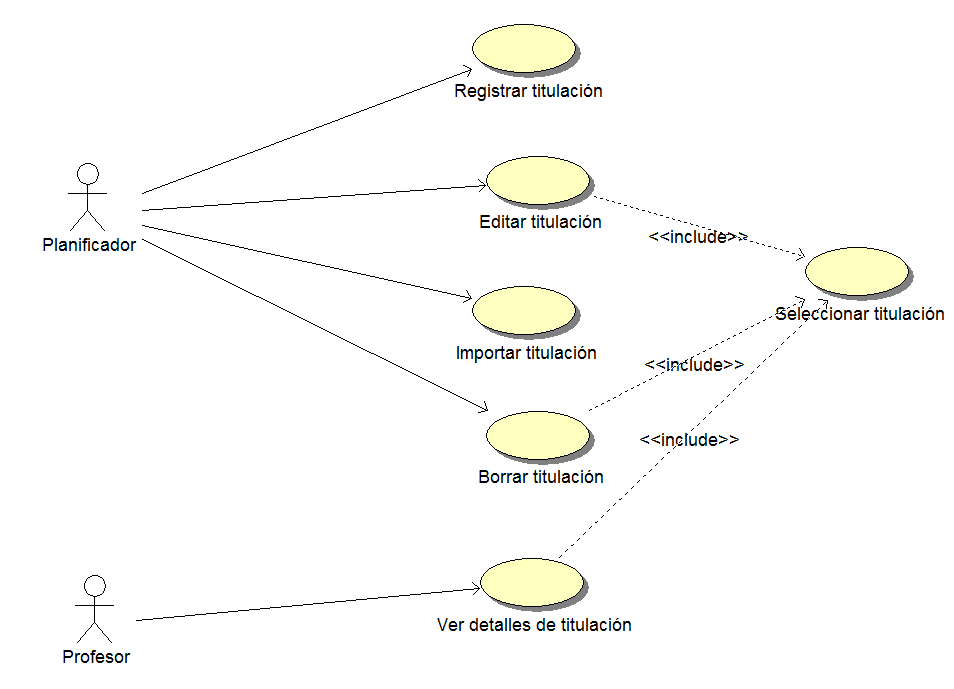
\includegraphics[scale=0.5]{./gestiontitulaciones.png}
  \end{center}
\caption{Diagrama de casos de uso de la gestión de titulaciones}
\end{figure}
\subsubsection*{Caso de uso: Seleccionar titulación}
\label{select_titulacion}
\begin{itemize}
\item{\bf Descripción:} Caso de uso abstracto incluído en otros casos de uso para seleccionar una titulación de una lista de disponibles.
\item{\bf Actores:} Usuario
\item{\bf Precondiciones:} Ninguna.
\item{\bf Postcondiciones:} Se selecciona una titulación para su uso en otra finalidad.
\item{\bf Escenario principal:}
\begin{enumerate}
\item El sistema muestra un listado de las titulaciones disponibles.
\item El usuario selecciona la titulación deseada.
\end{enumerate}
\item{\bf Escenarios alternativos:}
\begin{itemize}
\item[1.a.] No hay ninguna titulación registrada.
\begin{enumerate}
\item El sistema indica el error y el caso de uso finaliza.
\end{enumerate}
\end{itemize}
\end{itemize}



\subsubsection*{Caso de uso: Registrar titulación}
\begin{itemize}
\item{\bf Descripción:} Registra una nueva titulación en el sistema.
\item{\bf Actores:} Administrador.
\item{\bf Precondiciones:} Ninguna.
\item{\bf Postcondiciones:} La titulación queda registrada.
\item{\bf Escenario principal:}
\begin{enumerate}
\item El administrador introduce el código, el nombre y todos los demás datos de la titulación.
\item El sistema comprueba que los datos cumplen el formato.
\item El sistema confirma el alta de la titulación mostrando un mensaje.
\end{enumerate}
\item{\bf Escenarios alternativos:}
	\begin{itemize}
	\item[2.a.] Alguno de los datos introducidos tiene un formato incorrecto.
		\begin{enumerate}
		\item El sistema lo indica mostrando un mensaje de error y se vuelve al paso anterior.
		\end{enumerate}
	\item[2.b.] Falta algún campo obligatorio.
		\begin{enumerate}
		\item El sistema lo indica mostrando un mensaje de error y se vuelve al paso anterior.
		\end{enumerate}
	\item[2.c.] Ya existe alguna titulación con ese código o nombre.
		\begin{enumerate}
		\item El sistema indica el error y se vuelve al paso anterior.
		\end{enumerate}
	\item[*a.] El administrador decide cancelar el registro en cualquier momento, el caso de uso termina. 
	\end{itemize}
\end{itemize}



\subsubsection*{Caso de uso: Editar titulación}
\begin{itemize}
\item{\bf Descripción:} Edita una titulación existente en el sistema modificando sus datos.
\item{\bf Actores:} Administrador.
\item{\bf Precondiciones:} Ninguna.
\item{\bf Postcondiciones:} La titulacion queda modificada en el sistema.
\item{\bf Escenario principal:}
\begin{enumerate}
	\item Se realiza el caso de uso {\em\hyperref[select_titulacion]{Seleccionar titulación}}.
	\item El sistema muestra sus datos actuales, permitiendo su edición.
	\item El administrador modifica los datos.
	\item El sistema comprueba que todos los datos son correctos.
	\item El sistema muestra un mensaje indicando que la edición se ha completado.
\end{enumerate}
\item{\bf Escenarios alternativos:}
	\begin{itemize}
	\item[4.a.] Alguno de los datos tiene un formato incorrecto.
		\begin{enumerate}
		\item El sistema muestra un mensaje de error indicándolo, a continuación se vuelve al paso anterior.
		\end{enumerate}
	\item[4.b.] Falta algún campo obligatorio por rellenar.
		\begin{enumerate}
		\item El sistema muestra un mensaje de error indicándolo, a continuación se vuelve al paso anterior.
		\end{enumerate}
	\item[4.c.] Ya existe alguna titulación con el nombre o código introducidos.
		\begin{enumerate}
		\item El sitema indica el error y se vuelve al paso anterior.
		\end{enumerate}
	\item[*a.] En cualquier momento el administrador decide cancelar la edición, el caso de uso se da por terminado.
	\end{itemize}
\end{itemize}



\subsubsection*{Caso de uso: Borrar titulación}
% Tomar este CU como ejemplo
\begin{itemize}
\item{\bf Descripción:} Borra una titulación del sistema.
\item{\bf Actores:} Administrador.
\item{\bf Precondiciones:} La titulación existe en el sistema.
\item{\bf Postcondiciones:} La titulación queda eliminada del sistema.
\item{\bf Escenario principal:}
	\begin{enumerate}
	\item Se realiza el caso de uso  {\em\hyperref[select_titulacion]{Seleccionar titulación}}.
	\item El sistema muestra un diálogo de confirmación.
	\item El administrador confirma que quiere eliminar la titulación del sistema.
	\item El sistema elimina la titulación.
	\item El sistema muestra un mensaje confirmando que se ha eliminado la titulación.
	\end{enumerate}
\item{\bf Escenarios alternativos:}
	\begin{itemize}
	\item[3.a.] El administrador selecciona que no desea eliminar la titulación.
		\begin{enumerate}
		\item El caso de uso se reinicia.
		\end{enumerate}
	\item[*a.] En cualquier momento el administrador decide cancelar la eliminación.
		\begin{enumerate}
		\item El caso de uso se termina.
		\end{enumerate}
	\end{itemize}
\end{itemize}



\subsubsection*{Caso de uso: Ver detalles de titulación}
\begin{itemize}
\item{\bf Descripción:} Muestra los datos de una titulación en detalle, así como sus asignaturas.
\item{\bf Actores:} Usuario.
\item{\bf Precondiciones:} La titulación existe en el sistema.
\item{\bf Postcondiciones:} Los datos de la titulación se muestran por pantalla.
\item{\bf Escenario principal:}
	\begin{enumerate}
	\item Se realiza el caso de uso {\em\hyperref[select_titulacion]{Seleccionar titulación}}.
	\item El sistema muestra los datos de la titulación y un listado de sus asignaturas si las tiene.
	\end{enumerate}
\item{\bf Escenarios alternativos:}
	\begin{itemize}
	\item[*a.] En cualquier momento el usuario decide cancelar el proceso, el caso de uso se termina.
	\end{itemize}
\end{itemize}





\subsubsection*{Caso de uso: Importar titulación}
\begin{itemize}
\item{\bf Descripción:} Caso de uso para importar titulaciones de forma masiva desde un archivo csv con un formato concreto.
\item{\bf Actores:} Administrador
\item{\bf Precondiciones:} El archivo tiene el formato correcto.
\item{\bf Postcondiciones:} Se crean las titulaciones indicadas en el archivo.
\item{\bf Escenario principal:}
	\begin{enumerate}
	\item El administrador selecciona el archivo.
	\item El sistema comprueba que cada línea tenga el formato correcto.
	\item El sistema crea una titulación por cada línea con los datos indicados en el archivo.
	\end{enumerate}
\item{\bf Escenarios alternativos:}
	\begin{itemize}
		\item[2.a.] Alguna línea no cumple el formato
		\begin{enumerate}
			\item El sistema indica el error y el caso de uso finaliza.
		\end{enumerate}
		\item[2.b.] Ya existe una titulación creada con el mismo identificador.
		\begin{enumerate}
			\item El sistema lo indica y el caso de uso finaliza.
		\end{enumerate}
	\end{itemize}
\end{itemize}



\subsubsection{Gestión de asignaturas}
% Aquí va el diagrama de la gestión de asignaturas
\begin{figure}[H] 
  \label{gestion-asignaturas} 
	\begin{center}
    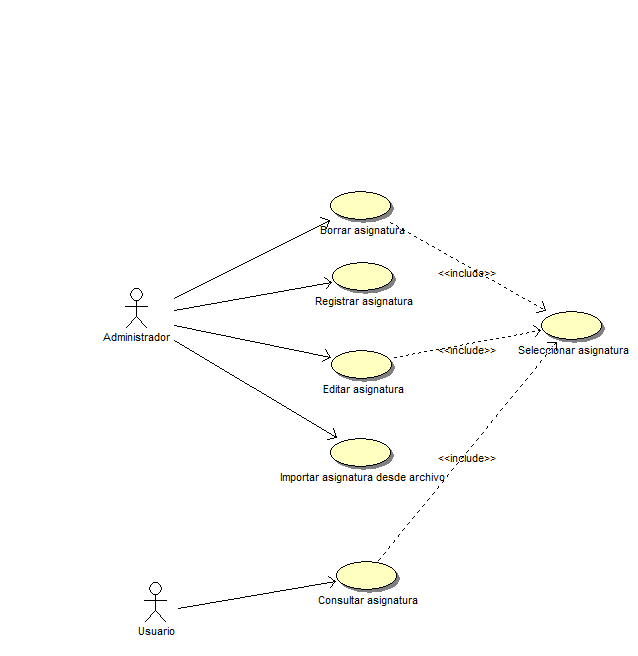
\includegraphics[scale=0.5]{./gestionasignaturas.png}
  \end{center}
\caption{Diagrama de casos de uso de la gestión de asignaturas}
\end{figure}
\subsubsection*{Caso de uso: Seleccionar asignatura}
\label{select_asignatura}
\begin{itemize}
\item{\bf Descripción:} Caso de uso abstracto incluído por otros casos de uso para seleccionar una asignatura del listado de las que tiene disponibles una titulación concreta.
\item{\bf Actores:} Usuario
\item{\bf Precondiciones:} Ninguna.
\item{\bf Postcondiciones:} Queda seleccionada una asignatura para algún fin concreto de otro caso de uso.
\item{\bf Escenario principal:}
	\begin{enumerate}
	\item Se realiza el caso de uso {\em\hyperref[select_titulacion]{Seleccionar titulación}}.
	\item El sistema muestra un listado de las asignaturas disponibles asociadas a la titulación seleccionada.
	\item El usuario selecciona una asignatura de la lista.
	\end{enumerate}
\item{\bf Escenarios alternativos:}
	\begin{itemize}
		\item[2.a.] No hay ninguna asignatura registrada en esa titulación.
		\begin{enumerate}
			\item El sistema indica el error y el caso de uso finaliza.
		\end{enumerate}
	\end{itemize}
\end{itemize}



\subsubsection*{Caso de uso: Registrar asignatura}
\begin{itemize}
\item{\bf Descripción:} Se da de alta una nueva asignatura en el sistema.
\item{\bf Actores:} Administrador.
\item{\bf Precondiciones:} Existe alguna titulación con la que asociar la asignatura.
\item{\bf Postcondiciones:} La asignatura queda registrada en el sistema.
\item{\bf Escenario principal:}
	\begin{enumerate}
 	\item Se realiza el caso de uso {\em\hyperref[select_titulacion]{Seleccionar titulación}}.
	\item El sistema muestra un formulario para introducir los datos.
	\item El administrador introduce el código, el nombre y todos los demás datos de la asignatura.
	\item El sistema comprueba que todos los datos cumplen el formato requerido.
	\item El sistema registra la asignatura y muestra un mensaje confirmándolo.
	\end{enumerate}
\item{\bf Escenarios alternativos:}
	\begin{itemize}
	\item[3.a.] El administrador selecciona que desea tomar los datos de otra asignatura.
		\begin{enumerate}
		\item Se realiza el caso de uso {\em \hyperref[duplicar_asignatura]{Duplicar asignatura}}.
		\end{enumerate}
	\item[4.a.] Alguno de los datos no cumple el formato correcto.
		\begin{enumerate}
		\item El sistema indica el error y se vuelve al paso anterior.
		\end{enumerate}
	\item[4.b.] Falta por rellenar algún campo obligatorio.
		\begin{enumerate}
		\item El sistema indica el error y se vuelve al paso anterior.
		\end{enumerate}
	\item[4.c.] Ya existe alguna asignatura con ese código o nombre.
		\begin{enumerate}
		\item El sistema indica el error y se vuelve al paso anterior.
		\end{enumerate}
	\item[*a.] En cualquier momento el administrador decide cancelar el proceso.
		\begin{enumerate}
		\item El caso de uso se cancela.
		\end{enumerate}
	\end{itemize}
\end{itemize}



\subsubsection*{Caso de uso: Editar Asignatura}
\begin{itemize}
\item{\bf Descripción:} Se modifican los datos de una asignatura existente en el sistema.
\item{\bf Actores:} Administrador.
\item{\bf Precondiciones:} Ninguna.
\item{\bf Postcondiciones:} La asignatura queda modificada en el sistema.
\item{\bf Escenario principal:}
	\begin{enumerate}
	\item Se realiza el caso de uso {\em \hyperref[select_asignatura]{Seleccionar asignatura}}.
	\item El sistema muestra los datos de la asignatura en un formato editable.
	\item El administrador hace las modificaciones que considere necesarias.
	\item El sistema comprueba que los datos modificados cumplen el formato requerido.
	\item El sistema guarda la asignatura y muestra un mensaje confirmándolo.
	\end{enumerate}
\item{\bf Escenarios alternativos:}
	\begin{itemize}
	\item[4.a.] Alguno de los datos no cumple el formato correcto.
		\begin{enumerate}
		\item El sistema indica el error y se vuelve al paso anterior.
		\end{enumerate}
	\item[4.b.] Falta por rellenar algún campo obligatorio.
		\begin{enumerate}
		\item El sistema indica el error y se vuelve al paso anterior.
		\end{enumerate}
	\item[4.c.] Ya existe alguna asignatura con ese código o nombre.
		\begin{enumerate}
		\item El sistema indica el error y se vuelve al paso anterior.
		\end{enumerate}
	\item[*a.] En cualquier momento el administrador decide cancelar el proceso.
		\begin{enumerate}
		\item El caso de uso se cancela.
		\end{enumerate}
	\end{itemize}
\end{itemize}



\subsubsection*{Caso de uso: Borrar asignatura}
\begin{itemize}
\item{\bf Descripción:} Se borra una asingatura del sistema.
\item{\bf Actores:} Administrador.
\item{\bf Precondiciones:} Ninguna.
\item{\bf Postcondiciones:} La asignatura queda eliminada del sistema.
\item{\bf Escenario principal:}
	\begin{enumerate}
	\item Se realiza el caso de uso {\em \hyperref[select_asignatura]{Seleccionar asignatura}}.
	\item El sistema muestra un diálogo de confirmación.
	\item El administrador confirma que desea borrar la asignatura.
	\item El sistema borra la asignatura y muestra un mensaje confirmándolo.
	\end{enumerate}
\item{\bf Escenarios alternativos:}
	\begin{itemize}
	\item[3.a.] El administrador selecciona que no desea eliminar la asignatura.
		\begin{enumerate}
		\item El caso de uso se reinicia.
		\end{enumerate}
	\item[*a.] En cualquier momento el administrador decide cancelar la eliminación.
		\begin{enumerate}
		\item El caso de uso se termina.
		\end{enumerate}
	\end{itemize}
\end{itemize}



\subsubsection*{Caso de uso: Consultar asignatura}
\begin{itemize}
\item{\bf Descripción:} Muestra los datos en detalle de una asignatura.
\item{\bf Actores:} Usuario.
\item{\bf Precondiciones:} Ninguna.
\item{\bf Postcondiciones:} Se muestran los datos de la asignatura por pantalla.
\item{\bf Escenario principal:} 
	\begin{enumerate}
	\item Se realiza el caso de uso {\em \hyperref[select_asignatura]{Seleccionar asignatura}}.
	\item El sistema muestra la información relacionada con la asignatura.
	\end{enumerate}
\item{\bf Escenarios alternativos:}
	\begin{itemize}
	\item[*a.] En cualquier momento el administrador decide cancelar el proceso.
		\begin{enumerate}
		\item El caso de uso se termina.
		\end{enumerate}
	\end{itemize}
\end{itemize}


\subsubsection*{Caso de uso: Importar asignatura desde archivo}
\begin{itemize}
\item{\bf Descripción:} Caso de uso para importar asignaturas de forma masiva desde un archivo csv con un formato concreto.
\item{\bf Actores:} Administrador
\item{\bf Precondiciones:} El archivo tiene el formato correcto.
\item{\bf Postcondiciones:} Se crean las asignaturas indicadas en el archivo.
\item{\bf Escenario principal:}
	\begin{enumerate}
	\item El administrador selecciona el archivo.
	\item El sistema comprueba que cada línea tenga el formato correcto.
	\item El sistema crea una asignatura por cada línea con los datos indicados en el archivo.
	\end{enumerate}
\item{\bf Escenarios alternativos:}
	\begin{itemize}
		\item[2.a.] Alguna línea no cumple el formato
		\begin{enumerate}
			\item El sistema indica el error y el caso de uso finaliza.
		\end{enumerate}
		\item[2.b.] Ya existe una asignatura creada con el mismo identificador.
		\begin{enumerate}
			\item El sistema lo indica y el caso de uso finaliza.
		\end{enumerate}
	\end{itemize}
\end{itemize}


\subsubsection{Gestión de cursos}
\begin{figure}[H] 
  \label{gestion-cursos} 
	\begin{center}
    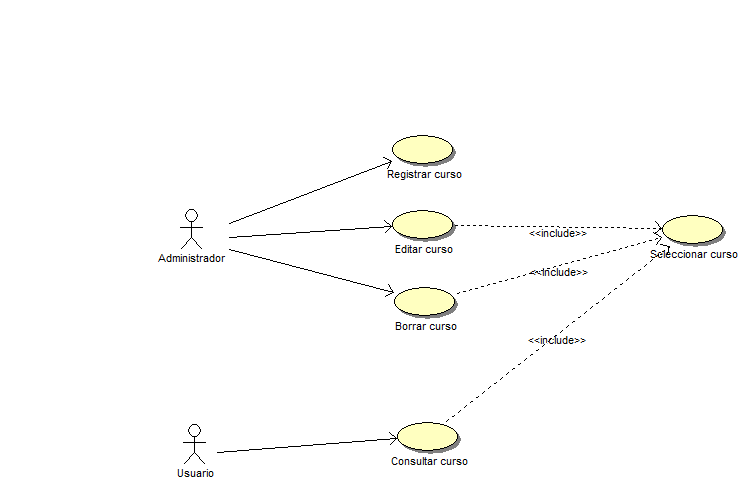
\includegraphics[scale=0.5]{./gestioncursos.png}
  \end{center}
\caption{Diagrama de casos de uso de la gestión de cursos}
\end{figure}

\subsubsection*{Caso de uso: Seleccionar curso}
\begin{itemize}
\item{\bf Descripción:} Caso de uso abstracto que es incluído en otros casos de uso.
\item{\bf Actores:} Usuario.
\item{\bf Precondiciones:} Ninguna.
\item{\bf Postcondiciones:} Queda seleccionado un curso para su uso con algún fin.
\item{\bf Escenario principal:}
	\begin{enumerate}
	\item El sistema muestra un listado con los cursos disponibles.
        \item El usuario selecciona un curso.
	\end{enumerate}
\item{\bf Escenarios alternativos:}
	\begin{itemize}
	\item[1.a.]No hay ningún curso registrado en el sistema.
	  \begin{enumerate}
	  \item El sistema indica el error y el caso de uso finaliza.
	  \end{enumerate}
	\end{itemize}
\end{itemize}




\subsubsection*{Caso de uso: Registrar curso}
\begin{itemize}
\item{\bf Descripción:} Se da de alta en el sistema la configuración de un nuevo curso.
\item{\bf Actores:} Administrador.
\item{\bf Precondiciones:} Ninguna.
\item{\bf Postcondiciones:} Queda registrado en el sistema el curso.
\item{\bf Escenario principal:}
  \begin{enumerate}
  \item El administrador introduce los datos de configuración del curso, incluyendo fecha de inicio y final de curso.
  \item El sistema comprueba que los datos sean correctos.
  \item El sistema informa de que el curso ha sido registrado con éxito.
  \end{enumerate}
\item{\bf Escenarios alternativos:}
  \begin{itemize}
  \item[2.a.] Alguno de los datos introducidos no cumple el formato correcto.
    \begin{enumerate}
    \item El sistema indica el error y se vuelve al paso anterior.
    \end{enumerate}
  \item[2.b.] Ya existe un curso registrado que empieza o termina en el mismo año que el introducido.
    \begin{enumerate}
    \item El sistema indica el error y se vuelve al paso anterior.
    \end{enumerate}
  \item[2.c.] Los años introducidos de inicio y fin del curso no son consecutivos.
    \begin{enumerate}
    \item El sistema indica el error y se vuelve al paso anterior.
    \end{enumerate}
  \item[2.d.] Alguna de las fechas de exámenes introducidas no están comprendidas entre la duración del curso.
    \begin{enumerate}
    \item El sistema indica el error y se vuelve al paso anterior.
    \end{enumerate}
  \item[*a.] En cualquier momento el administrador decide cancelar el proceso.
    \begin{enumerate}
    \item El caso de uso finaliza.
    \end{enumerate}
  \end{itemize}
\end{itemize}



\subsubsection*{Caso de uso: Editar curso}
\begin{itemize}
\item{\bf Descripción:} Se edita en el sistema la configuración de un curso.
\item{\bf Actores:} Administrador.
\item{\bf Precondiciones:} Ninguna.
\item{\bf Postcondiciones:} Quedan registradas en el sistema las modificaciones realizadas.
\item{\bf Escenario principal:}
  \begin{enumerate}
  \item Se realiza el caso de uso {\em \hyperref[select_curso]{Seleccionar curso}}.
  \item El sistema muestra los datos en forma editable.
  \item El administrador modifica los datos de configuración del curso que considere necesarios.
  \item El sistema comprueba que los datos sean correctos.
  \item El sistema informa de que el curso ha sido registrado con éxito.
  \end{enumerate}
\item{\bf Escenarios alternativos:}
  \begin{itemize}
  \item[4.a.] Alguno de los datos introducidos no cumple el formato correcto.
    \begin{enumerate}
    \item El sistema indica el error y se vuelve al paso anterior.
    \end{enumerate}
  \item[4.b.] Ya existe un curso registrado que empieza o termina en el mismo año que el introducido.
    \begin{enumerate}
    \item El sistema indica el error y se vuelve al paso anterior.
    \end{enumerate}
  \item[4.c.] Los años introducidos de inicio y fin del curso no son consecutivos.
    \begin{enumerate}
    \item El sistema indica el error y se vuelve al paso anterior.
    \end{enumerate}
  \item[4.d.] Alguna de las fechas de exámenes introducidas no están comprendidas entre la duración del curso.
    \begin{enumerate}
    \item El sistema indica el error y se vuelve al paso anterior.
    \end{enumerate}
  \item[*a.] En cualquier momento el administrador decide cancelar el proceso.
    \begin{enumerate}
    \item El caso de uso finaliza.
    \end{enumerate}
  \end{itemize}
\end{itemize}



\subsubsection*{Caso de uso: Consultar curso}
\begin{itemize}
\item{\bf Descripción:} Se consulta la configuración de un curso mostrandola por pantalla
\item{\bf Actores:} Usuario.
\item{\bf Precondiciones:} Ninguna.
\item{\bf Postcondiciones:} Se muestra por pantalla la configuración del curso seleccionado.
\item{\bf Escenario principal:}
  \begin{enumerate}
  \item Se realiza el caso de uso {\em \hyperref[select_curso]{Seleccionar curso}}.
  \item El sistema muestra los datos del curso.
  \end{enumerate}
\item{\bf Escenarios alternativos:}
  \begin{itemize}
  \item[*a.] En cualquier momento el administrador decide cancelar el proceso.
    \begin{enumerate}
    \item El caso de uso finaliza.
    \end{enumerate}
  \end{itemize}
\end{itemize}



\subsubsection*{Caso de uso: Borrar curso}
\begin{itemize}
\item{\bf Descripción:} Se elimina un curso registrado en el sistema.
\item{\bf Actores:} Administrador
\item{\bf Precondiciones:} Ninguna
\item{\bf Postcondiciones:} El curso seleccionado queda eliminado del sistema
\item{\bf Escenario principal:}
	\begin{enumerate}
	\item Se realiza el caso de uso {\em \hyperref[select_curso]{Seleccionar curso}}.
	\item El sistema muestra un diálogo pidiendo la confirmación del borrado.
	\item El administrador selecciona que desea confirmar el borrado.
	\item El sistema muestra un mensaje confirmando el éxito en la operación.
	\end{enumerate}
\item{\bf Escenarios alternativos:}
	\begin{itemize}
		\item[3.a.] El administrador selecciona que no desea confirmar el borrado.
		\begin{enumerate}
			\item El caso de uso se reinicia.
		\end{enumerate}
		\item[*a.] En cualquier momento el administrador cancela el proceso.
		\begin{enumerate}
			\item El caso de uso finaliza.
		\end{enumerate}
	\end{itemize}
\end{itemize}


\subsubsection{Gestión de planificación docente}
\begin{figure}[H] 
  \label{gestion-planificacion} 
	\begin{center}
    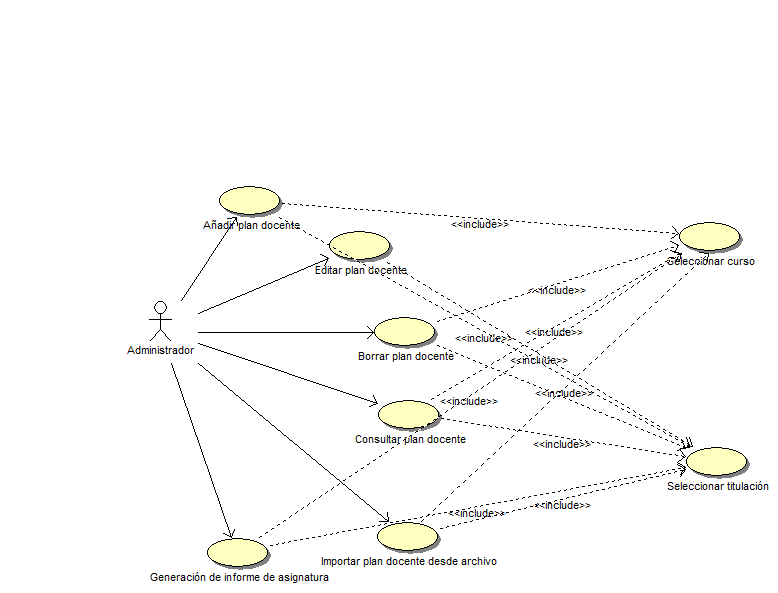
\includegraphics[scale=0.5]{./gestionplanificacion.png}
  \end{center}
\caption{Diagrama de casos de uso de la gestión de la planificación docente}
\end{figure}
\subsubsection*{Caso de uso: Añadir plan docente}
\begin{itemize}
\item{\bf Descripción:} Se añaden los detalles del plan docente para una asignatura en un curso determinado.
\item{\bf Actores:} Subdirector.
\item{\bf Precondiciones:} Ninguna.
\item{\bf Postcondiciones:} El plan docente queda registrado en el sistema, asociado a una asignatura y un curso determinado.
\item{\bf Escenario principal:}
	\begin{enumerate}
	\item Se realiza el caso de uso {\em \hyperref[select_asignatura]{Seleccionar asignatura}}.
	\item Se realiza el caso de uso {\em \hyperref[select_curso]{Seleccionar curso}}.
	\item El sistema comprueba que no exista ya un plan docente asociado a ese curso.
	\item El usuario introduce los datos del plan docente.
	\item El sistema comprueba que los datos cumplen el formato requerido.
	\item El sistema guarda la carga de trabajo y muestra un mensaje confirmándolo.
	\end{enumerate}
\item{\bf Escenarios alternativos:}
	\begin{itemize}
	\item[3.a.] Ya existe una carga de trabajo establecida para el curso seleccionado.
		\begin{enumerate}
		\item El sistema indica el error y el caso de uso vuelve al paso anterior.
		\end{enumerate}
	\item[4.a.] El usuario indica que quiere tomar los datos de otra carga de un curso anterior.
		\begin{enumerate}
		\item Se realiza el caso de uso {\em \hyperref[duplicar_carga]{Duplicar carga de trabajo}}
		\end{enumerate}
	\item[5.a.] Alguno de los datos introducidos no cumple el formato correcto.
		\begin{enumerate}
		\item El sistema indica el error y se vuelve al paso anterior.
		\end{enumerate}
	\item[5.b.] Alguno de los campos obligatorios no ha sido rellenado.
		\begin{enumerate}
		\item El sistema indica el error y se vuelve al paso anterior.
		\end{enumerate}	
	\item[*a.] En cualquier momento el administrador decide cancelar el proceso.
		\begin{enumerate}
		\item El caso de uso se termina.
		\end{enumerate}
	\end{itemize}
\end{itemize}



\subsubsection*{Caso de uso: Editar plan docente}
\begin{itemize}
\item{\bf Descripción:} Se edita una carga de trabajo existente para un curso determinado.
\item{\bf Actores:} Subdirector.
\item{\bf Precondiciones:} Ninguna.
\item{\bf Postcondiciones:} La carga de trabajo queda modificada en el sistema.
\item{\bf Pasos:}
	\begin{enumerate}
	\item Se realiza el caso de uso {\em \hyperref[select_asignatura]{Seleccionar asignatura}}.
	\item Se realiza el caso de uso {\em \hyperref[select_curso]{Seleccionar curso}}.
	\item El sistema comprueba que exista una carga asociada a ese curso.
	\item El sistema muestra los datos de la carga en un formato editable.
	\item El usuario modifica los datos.
	\item El sistema comprueba que los datos cumplen el formato requerido.
	\item El sistema guarda los cambios y muestra un mensaje confirmándolo.
	\end{enumerate}
\item{\bf Escenarios alternativos:}
	\begin{itemize}
	\item[3.a.] No existe una carga de trabajo establecida para el curso seleccionado.
		\begin{enumerate}
		\item El sistema indica el error y el caso de uso vuelve al paso anterior.
		\end{enumerate}
	\item[5.a.] Alguno de los datos introducidos no cumple el formato correcto.
		\begin{enumerate}
		\item El sistema indica el error y se vuelve al paso anterior.
		\end{enumerate}
	\item[5.b.] Alguno de los campos obligatorios no ha sido rellenado.
		\begin{enumerate}
		\item El sistema indica el error y se vuelve al paso anterior.
		\end{enumerate}	
	\item[*a.] En cualquier momento el administrador decide cancelar el proceso.
		\begin{enumerate}
		\item El caso de uso se termina.
		\end{enumerate}
	\end{itemize}
\end{itemize}



\subsubsection*{Caso de uso: Borrar plan docente}
\begin{itemize}
\item{\bf Descripción:} Se borra una carga de trabajo existente en el sistema asociada a un curso.
\item{\bf Actores:} Subdirector.
\item{\bf Precondiciones:} Ninguna.
\item{\bf Postcondiciones:} La carga de trabajo asociada a la asignatura y curso seleccionados queda. eliminada del sistema.
\item{\bf Escenario principal:}
	\begin{enumerate}
	\item Se realiza el caso de uso {\em \hyperref[select_asignatura]{Seleccionar asignatura}}
	\item Se realiza el caso de uso {\em \hyperref[select_curso]{Seleccionar curso}}.
	\item El sistema comprueba que exista una carga asociada a ese curso.
	\item El sistema muestra un diálogo de confirmación.
	\item El usuario confirma que desea borrar la carga.
	\item El sistema muestra un mensaje confirmando la eliminación y borra la carga.
	\end{enumerate}
\item{\bf Escenarios alternativos:}
	\begin{itemize}
	\item[3.a.] No existe una carga de trabajo establecida para el curso seleccionado.
	  \begin{enumerate}
	  \item El sistema indica el error y el caso de uso vuelve al paso anterior.
	  \end{enumerate}
	\item[5.a.] El administrador selecciona que no desea eliminar la carga.
		\begin{enumerate}
		\item El caso de uso se reinicia.
		\end{enumerate}
	\item[*a.] En cualquier momento el administrador decide cancelar la eliminación.
		\begin{enumerate}
		\item El caso de uso se termina.
		\end{enumerate}
	\end{itemize}
\end{itemize}



\subsubsection*{Caso de uso: Consultar plan docente}
\begin{itemize}
\item{\bf Descripción:} Se consulta la carga de trabajo de una asignatura para un curso determinado.
\item{\bf Actores:} Usuario.
\item{\bf Precondiciones:} Ninguna.
\item{\bf Postcondiciones:} Se muestran los datos al usuario por pantalla.
\item{\bf Escenario principal:}
	\begin{enumerate}
	\item Se realiza el caso de uso {\em \hyperref[select_asignatura]{Seleccionar asignatura}}
	\item Se realiza el caso de uso {\em \hyperref[select_curso]{Seleccionar curso}}.
	\item El sistema comprueba que exista una carga asociada a ese curso.
	\item La carga existe y es mostrada al usuario.
	\end{enumerate}
\item{\bf Escenarios alternativos:}
	\begin{itemize}
	\item[3.a.]No existe ninguna carga asociada a ese curso.
		\begin{enumerate}
		\item El sistema muestra un mensaje informando del error y vuelve al paso anterior.
		\end{enumerate}
	\item[*a.]En cualquier momento el usuario decide cancelar el proceso.
		\begin{enumerate}
		\item El caso de uso se cancela.
		\end{enumerate}		
	\end{itemize}
\end{itemize}




\subsubsection*{Caso de uso: Importar plan docente desde archivo}
\begin{itemize}
\item{\bf Descripción:} Caso de uso para importar planes docentes de forma masiva desde un archivo csv con un formato concreto.
\item{\bf Actores:} Administrador
\item{\bf Precondiciones:} El archivo tiene el formato correcto.
\item{\bf Postcondiciones:} Se crean los planes docentes indicados en el archivo.
\item{\bf Escenario principal:}
	\begin{enumerate}
	\item El administrador selecciona el archivo.
	\item El sistema comprueba que cada línea tenga el formato correcto.
	\item El sistema crea un plan docente por cada línea con los datos indicados en el archivo.
	\end{enumerate}
\item{\bf Escenarios alternativos:}
	\begin{itemize}
		\item[2.a.] Alguna línea no cumple el formato
		\begin{enumerate}
			\item El sistema indica el error y el caso de uso finaliza.
		\end{enumerate}
		\item[2.b.] Ya existe un plan docente creado para la asignatura indicada y para ese curso.
		\begin{enumerate}
			\item El sistema lo indica y el caso de uso finaliza.
		\end{enumerate}
	\end{itemize}
\end{itemize}


\subsubsection*{Caso de uso: Generación de informe de asignatura}
\begin{itemize}
\item{\bf Descripción:} Caso de uso para generar un informe de las horas asignadas a una asignatura.
\item{\bf Actores:} Administrador
\item{\bf Precondiciones:} La asignatura tiene un plan docente creado y asignadas horas en los horarios.
\item{\bf Postcondiciones:} Se genera un informe en pdf permitiendo su descarga.
\item{\bf Escenario principal:}
	\begin{enumerate}
	\item Se realiza el caso de uso {\em \hyperref[select_curso]{Seleccionar curso}}.
	\item Se realiza el caso de uso {\em \hyperref[select_asignatura]{Seleccionar asignatura}}.
	\item El sistema comprueba el plan docente de la asignatura y las asignaciones en los horarios.
	\item El sistema muestra un desglose de las horas de cada actividad de la asignatura y de cada semana teniendo en cuenta los eventos del calendario, permitiendo la descarga del archivo.
	\end{enumerate}
\item{\bf Escenarios alternativos:}
	\begin{itemize}
		\item[*.a.] En cualquier momento se decide parar el proceso.
		\begin{enumerate}
			\item El caso de uso finaliza.
		\end{enumerate}
		\item[3.a] La asignatura no tiene un plan docente asignado.
		\begin{enumerate}
			\item El caso de uso finaliza.
		\end{enumerate}
	\end{itemize}
\end{itemize}

\subsubsection{Gestión del calendario}
\begin{figure}[H] 
  \label{gestion-calendario} 
	\begin{center}
    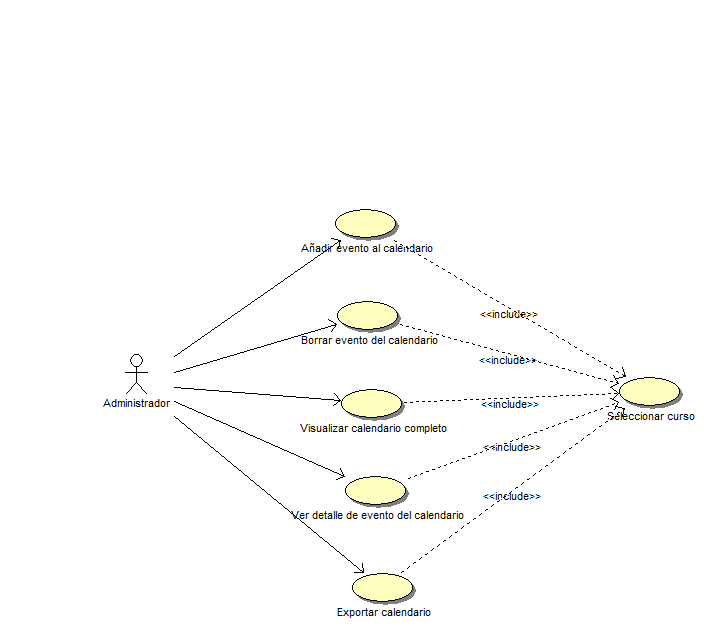
\includegraphics[scale=0.5]{./gestioncalendario.png}
  \end{center}
\caption{Diagrama de casos de uso de la gestión del calendario}
\end{figure}


\subsubsection*{Caso de uso: Añadir evento al calendario}
\begin{itemize}
\item{\bf Descripción:} Añade un evento de fechas al calendario, que puede ser una festividad o un período de vacaciones.
\item{\bf Actores:} Subdirector.
\item{\bf Precondiciones:} Ninguna.
\item{\bf Postcondiciones:} El evento queda registrado para el calendario de un curso concreto.
\item{\bf Escenario principal:}
	\begin{enumerate}
	\item Se realiza el caso de uso {\em \hyperref[select_curso]{Seleccionar curso}}.
	\item El subdirector introduce los datos correspondientes al evento, que serían, el nombre del evento, el tipo de evento, si es una fecha concreta o un rango de ellas, y su fecha de inicio y finalización.
	\item El sistema comprueba que los datos son correctos y que no se solapen con otros eventos.
	\item El sistema indica que todo es correcto y muestra un mensaje confirmando el éxito de la operación.
	\end{enumerate}
\item{\bf Escenarios alternativos:}
	\begin{itemize}
		\item[3.a.] Alguno de los datos tiene un formato incorrecto o algún campo está en blanco.
		\begin{enumerate}
			\item El sistema lo indica y vuelve al paso anterior.
		\end{enumerate}
		\item[3.b.] Las fechas del evento se solapan con algún otro evento o fecha del curso.
		\begin{enumerate}
			\item El sistema lo indica y vuelve al paso anterior.
		\end{enumerate}
		\item[*a.] En cualquier momento el usuario decide cancelar el proceso.
		\begin{enumerate}
		\item El caso de uso finaliza.
		\end{enumerate}
	\end{itemize}
\end{itemize}



\subsubsection*{Caso de uso: Borrar evento del calendario}
\begin{itemize}
\item{\bf Descripción:} El usuario selecciona alguno de los eventos del calendario para eliminarlo y este queda eliminado del sistema.
\item{\bf Actores:} Subdirector.
\item{\bf Precondiciones:} Ninguna.
\item{\bf Postcondiciones:} El evento queda eliminado del calendario del curso concreto.
\item{\bf Escenario principal:}
	\begin{enumerate}
	\item Se realiza el caso de uso {\em \hyperref[select_curso]{Seleccionar curso}}.
	\item El sistema muestra un listado de fechas de eventos.
	\item El subdirector selecciona la fecha que desea eliminar.
	\item El sistema muestra un mensaje confirmando que el evento ha sido eliminado.
	\end{enumerate}
\item{\bf Escenarios alternativos:}
	\begin{itemize}
		\item[2.a.] No hay ningún evento registrado en el calendario de ese curso.
		\begin{enumerate}
			\item El sistema lo indica y el caso de uso finaliza.
		\end{enumerate}
		\item[*a.] En cualquier momento el subdirector decide cancelar el proceso.
		\begin{enumerate}
		\item El caso de uso finaliza sin eliminar el evento.
		\end{enumerate}
	\end{itemize}
\end{itemize}



\subsubsection*{Caso de uso: Visualizar calendario completo}
\begin{itemize}
\item{\bf Descripción:} Se muestra un calendario completo con las fechas marcadas.
\item{\bf Actores:} Usuario.
\item{\bf Precondiciones:} Ninguna.
\item{\bf Postcondiciones:} Se muestra el calendario por pantalla.
\item{\bf Escenario principal:}
	\begin{enumerate}
	\item Se realiza el caso de uso {\em \hyperref[select_curso]{Seleccionar curso}}.
	\item El sistema muestra un calendario con las fechas de los eventos marcadas.
	\end{enumerate}
\item{\bf Escenarios alternativos:}
\end{itemize}


\subsubsection*{Caso de uso: Ver detalle de evento del calendario}
\begin{itemize}
\item{\bf Descripción:} Se muestran los datos detallados de un evento del calendario
\item{\bf Actores:} Usuario
\item{\bf Precondiciones:} Hay eventos registrados en el sistema
\item{\bf Postcondiciones:} Se muestran los datos.
\item{\bf Escenario principal:}
	\begin{enumerate}
	\item Se realiza el caso de uso {\em \hyperref[select_curso]{Seleccionar curso}}.
	\item El sistema muestra el calendario para el curso actual con los eventos creados sobre él.
	\item El usuario selecciona un evento
	\item El sistema muestra los datos del evento, título, razón, etc.
	\end{enumerate}
\item{\bf Escenarios alternativos:}
\end{itemize}




\subsubsection*{Caso de uso: Exportar calendario}
\begin{itemize}
\item{\bf Descripción:} Caso de uso para exportar el calendario de un curso a un formato externo como csv o una hoja de cálculo.
\item{\bf Actores:} Administrador.
\item{\bf Precondiciones:} El curso existe y tiene eventos creados.
\item{\bf Postcondiciones:} Se exporta un archivo con un formato adecuado.
\item{\bf Escenario principal:}
	\begin{enumerate}
	\item Se realiza el caso de uso {\em \hyperref[select_curso]{Seleccionar curso}}.
	\item Se muestra y permite descarga del archivo exportado.
	\end{enumerate}
\item{\bf Escenarios alternativos:}
	\begin{itemize}
		\item[*.a.] En cualquier momento el administrador decide cancelar el proceso.
		\begin{enumerate}
			\item Se finaliza el caso de uso.
		\end{enumerate}
	\end{itemize}
\end{itemize}


\subsubsection{Gestión de horarios}
\begin{figure}[H] 
  \label{gestion-horarios} 
	\begin{center}
    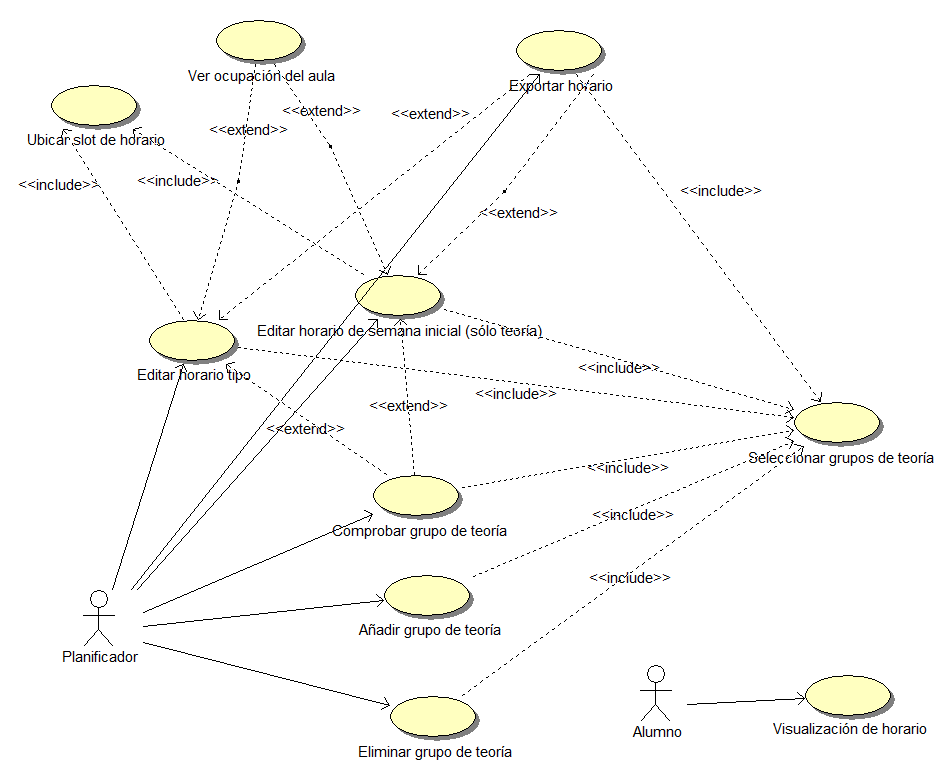
\includegraphics[scale=0.5]{./gestionhorarios.png}
  \end{center}
\caption{Diagrama de casos de uso de la gestión de titulaciones}
\end{figure}

\subsubsection*{Caso de uso: Seleccionar grupos de teoría}
\label{select_grupo}
\begin{itemize}
\item{\bf Descripción:} Se muestran los grupos de teoría de una titulación. Este caso de uso es incluido por más casos de uso.
\item{\bf Actores:} Administrador
\item{\bf Precondiciones:} Hay titulaciones y cursos creados.
\item{\bf Postcondiciones:} Se muestra la información
\item{\bf Escenario principal:}
	\begin{enumerate}
	\item Se realiza el caso de uso {\em \hyperref[select_curso]{Seleccionar curso}}.
	\item Se realiza el caso de uso {\em \hyperref[select_titulacion]{Seleccionar titulación}}.
	\item El sistema muestra un listado con los cursos de la titulación y el número de grupos de cada curso.
	\item El administrador selecciona el grupo deseado.
	\end{enumerate}
\item{\bf Escenarios alternativos:}
\end{itemize}



\subsubsection*{Caso de uso: Ubicar slot de horario}
\label{guardar_slot}
\begin{itemize}
\item{\bf Descripción:} Caso de uso abstracto que es incluído por otros casos de uso. Se utiliza para ubicar en un horario un slot de una actividad de una asignatura.
\item{\bf Actores:} Administrador
\item{\bf Precondiciones:} La asignatura existe y tiene asignadas horas en el plan docente para esa actividad.
\item{\bf Postcondiciones:} El slot de la actividad queda guardado en el horario.
\item{\bf Escenario principal:}
	\begin{enumerate}
	\item El administrador selecciona una asignatura y su actividad
	\item El sistema comprueba que tenga asignadas horas en el plan docente
	\item El administrador selecciona el aula en la que se guardará el slot
	\item El administrador selecciona el lugar que ocupará en el horario
	\item El sistema comprueba que el aula no esté ocupada en ese momento y que si el slot es de teoría que no se solape con otros slots.
	\item El sistema guarda el slot en el horario.
	\end{enumerate}
\item{\bf Escenarios alternativos:}
	\begin{itemize}
		\item[2.a.] La asignatura no tiene horas asignadas para esa actividad.
		\begin{enumerate}
			\item El sistema lo indica y se vuelve al paso anterior.
		\end{enumerate}
		\item[5.a.] El aula está ocupada en ese horario.
		\begin{enumerate}
			\item El sistema lo indica y se vuelve al paso 3.
		\end{enumerate}
		\item[5.b.] El slot es de teoría y se solapa con otros slots.
		\begin{enumerate}
			\item El sistema lo indica y se vuelve al paso anterior.
		\end{enumerate}
	\end{itemize}
\end{itemize}



\subsubsection*{Caso de uso: Editar horario tipo}
\begin{itemize}
\item{\bf Descripción:} Se muestra el horario de un grupo de teoría en un formato editable.
\item{\bf Actores:} Administrador
\item{\bf Precondiciones:} Hay algún grupo creado para la titulación, semestre, curso y año académico.
\item{\bf Postcondiciones:} Se muestran las asignaturas disponibles, permitiendo su edición. Se muestran tanto los slots de teoría como los de las demás actividades
\item{\bf Escenario principal:}
	\begin{enumerate}
	\item Se realiza el caso de uso {\em \hyperref[select_grupo]{Seleccionar grupos de teoría}}.
	\item El administrador selecciona el curso y semestre deseado para editar su horario tipo.
	\item El sistema comprueba que exista el grupo y se que no exista un horario ya empezado.
	\item Se realiza el caso de uso {\em \hyperref[guardar_slot]{Ubicar slot de horario}}.
	\item El administrador realiza el paso anterior las veces que sean necesarias hasta completar el horario.
	\end{enumerate}
\item{\bf Escenarios alternativos:}
	\begin{itemize}
		\item[*.a.] En cualquier momento el administrador decide parar el proceso.
		\begin{enumerate}
			\item El sistema guarda los cambios hechos hasta ahora y el caso de uso finaliza.
		\end{enumerate}
		\item[2.a] No ha sido creado ningún grupo para ese curso.
		\begin{enumerate}
			\item El sistema indica el error y finaliza el caso de uso.
		\end{enumerate}
		\item[3.a] Ya hay un horario empezado para ese grupo y semestre
		\begin{enumerate}
			\item El sistema muestra el horario ya empezado ubicando los slots donde estaban en el antiguo horario y el caso de uso continua.
		\end{enumerate}
	\end{itemize}
\end{itemize}



\subsubsection*{Caso de uso: Editar horario de semana inicial (sólo teoría)}
\begin{itemize}
\item{\bf Descripción:} Se muestra para su edición el horario de un grupo de teoría en una semana en la que sólo se imparte teoría
\item{\bf Actores:} Administrador
\item{\bf Precondiciones:} Ya ha sido creado el grupo y editado el horario tipo correspondiente
\item{\bf Postcondiciones:} Se muestra el horario con los slots de teoría del horario tipo ubicados en su sitio, salvo los que no sean posible por no ser día lectivo
\item{\bf Escenario principal:}
	\begin{enumerate}
	\item Se realiza el caso de uso {\em \hyperref[select_grupo]{Seleccionar grupo de teoría}}.
	\item El administrador selecciona el curso y semestre además de la semana que se editará.
	\item El sistema comprueba que exista el grupo y se que no exista un horario ya empezado.
	\item El sistema muestra los slots de teoría del horario tipo correspondiente, sacando del horario los que no sean posibles ubicar automáticamente por que el día sea no lectivo.
	\item Se realiza el caso de uso {\em \hyperref[guardar_slot]{Ubicar slot de horario}}.
	\item Se realiza el paso anterior las veces que se consideren necesarias hasta completar el horario.
	\end{enumerate}
\item{\bf Escenarios alternativos:}
	\begin{itemize}
		\item[*.a.] En cualquier momento el administrador decide parar el proceso.
		\begin{enumerate}
			\item El sistema guarda los cambios hechos hasta ahora y el caso de uso finaliza.
		\end{enumerate}
		\item[2.a] No ha sido creado ningún grupo para ese curso.
		\begin{enumerate}
			\item El sistema indica el error y finaliza el caso de uso.
		\end{enumerate}
		\item[3.a] Ya hay un horario empezado para ese grupo, semestre y semana
		\begin{enumerate}
			\item El sistema muestra el horario ya empezado ubicando los slots donde estaban en el antiguo horario y el caso de uso continua.
		\end{enumerate}
	\end{itemize}
\end{itemize}



\subsubsection*{Caso de uso: Añadir grupo de teoría}
\begin{itemize}
\item{\bf Descripción:} Se añade un grupo de teoría a un curso de una titulación para poder editar más adelante su horario
\item{\bf Actores:} Administrador
\item{\bf Precondiciones:} La titulación existe y tiene asignaturas con planes docentes creados para el curso actual.
\item{\bf Postcondiciones:} El grupo se añade al curso correspondiente.
\item{\bf Escenario principal:}
	\begin{enumerate}
	\item Se realiza el caso de uso {\em \hyperref[select_grupo]{Seleccionar grupo de teoría}}.
	\item El administrador selecciona el curso de la titulación al que se va a añadir el grupo.
	\item El sistema comprueba que no se haya sobrepasado el número de grupos indicado en el plan docente y guarda el grupo.
	\end{enumerate}
\item{\bf Escenarios alternativos:}
	\begin{itemize}
		\item[2.a.] Se han sobrepasado el número de grupos indicado en el plan docente.
		\begin{enumerate}
			\item El sistema advierte del problema pero el caso de uso continúa.
		\end{enumerate}
	\end{itemize}
\end{itemize}



\subsubsection*{Caso de uso: Eliminar grupo de teoría}
\begin{itemize}
\item{\bf Descripción:} Se elimina un grupo de teoría de un curso de una titulación
\item{\bf Actores:} Administrador
\item{\bf Precondiciones:} Hay grupos creados para la titulación y curso.
\item{\bf Postcondiciones:} Se elimina el grupo así como toda su información asociada (horarios, informes, etc).
\item{\bf Escenario principal:}
	\begin{enumerate}
	\item Se realiza el caso de uso {\em \hyperref[select_grupo]{Seleccionar grupo de teoría}}.
	\item El administrador selecciona el curso de la titulación al que se va a eliminar el grupo.
	\item El sistema pide confirmación de la eliminación.
	\item El administrador confirma que desea eliminar el grupo.
	\item Queda borrado el grupo y toda la información asociada y el sistema lo indica.
	\end{enumerate}
\item{\bf Escenarios alternativos:}
	\begin{itemize}
		\item[4.a.] El administrador cancela el proceso.
		\begin{enumerate}
			\item El caso de uso finaliza.
		\end{enumerate}
	\end{itemize}
\end{itemize}



\subsubsection*{Caso de uso: Exportar horario}
\begin{itemize}
\item{\bf Descripción:} Caso de uso para exportar un horario creado a un formato externo como csv o una hoja de cálculo.
\item{\bf Actores:} Administrador.
\item{\bf Precondiciones:} Existe un grupo creado y está creado el horario.
\item{\bf Postcondiciones:} Se exporta un archivo con un formato adecuado.
\item{\bf Escenario principal:}
	\begin{enumerate}
	\item Se realiza el caso de uso {\em \hyperref[select_grupo]{Seleccionar grupo de teoría}}.
	\item El administrador selecciona la semana, semestre y curso.
	\item El sistema busca el horario elegido.
	\item Se muestra y permite descarga del archivo exportado.
	\end{enumerate}
\item{\bf Escenarios alternativos:}
	\begin{itemize}
		\item[*.a.] En cualquier momento el administrador decide cancelar el proceso.
		\begin{enumerate}
			\item El caso de uso finaliza.
		\end{enumerate}
		\item[3.a.] No existe un horario creado para los datos elegidos.
		\begin{enumerate}
			\item El sistema lo indica y se vuelve al paso anterior.
		\end{enumerate}
	\end{itemize}
\end{itemize}


\subsubsection*{Caso de uso: Comprobar grupo de teoría}
\begin{itemize}
\item{\bf Descripción:} Caso de uso para comprobar que el número de horas introducidas en los horarios de un grupo coincide con lo indicado en el plan docente de cada asignatura.
\item{\bf Actores:} Administrador.
\item{\bf Precondiciones:} El grupo existe y tiene horarios creados.
\item{\bf Postcondiciones:} Se muestra la comprobación indicando si faltan o sobran horas en las asignaturas y actividades.
\item{\bf Escenario principal:}
	\begin{enumerate}
	\item Se realiza el caso de uso {\em \hyperref[select_grupo]{Seleccionar grupo de teoría}}.
	\item El sistema muestra el cálculo de horas de un grupo mediante los horarios de esa semana, teniendo en cuenta los eventos asignados en el calendario e indica dónde faltan horas por asignar para que sea solucionado.
	\end{enumerate}
\item{\bf Escenarios alternativos:}
	\begin{itemize}
		\item[*.a.] En cualquier momento se decide parar el proceso.
		\begin{enumerate}
			\item El caso de uso finaliza.
		\end{enumerate}
	\end{itemize}
\end{itemize}



\subsubsection{Gestión de aulas}
\begin{figure}[H] 
  \label{gestion-aulas} 
	\begin{center}
    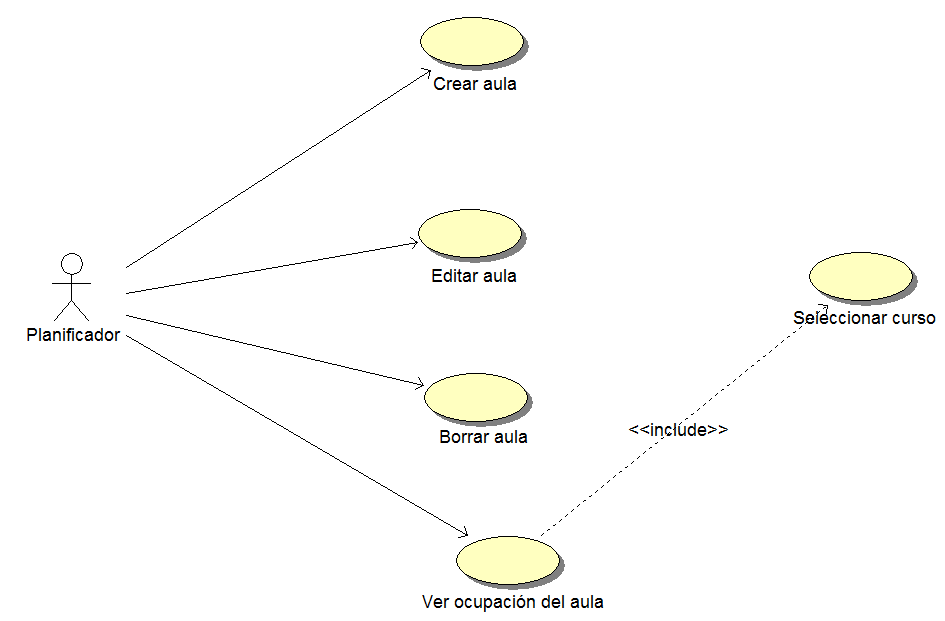
\includegraphics[scale=0.5]{./gestionaulas.png}
  \end{center}
\caption{Diagrama de casos de uso de la gestión de aulas}
\end{figure}
\subsubsection*{Caso de uso: Crear aula}
\begin{itemize}
\item{\bf Descripción:} Caso de uso para crear un aula a la que asignar slots de horario
\item{\bf Actores:} Administrador
\item{\bf Precondiciones:} Ninguna
\item{\bf Postcondiciones:} El aula queda creada
\item{\bf Escenario principal:}
	\begin{enumerate}
	\item El administrador introduce los datos del aula: nombre y actividades para las que sirve
	\item El sistema comprueba que no exista ningún aula con ese nombre y el aula queda creada.
	\end{enumerate}
\item{\bf Escenarios alternativos:}
	\begin{itemize}
		\item[*.a.] En cualquier momento el administrador decide cancelar el proceso.
		\begin{enumerate}
			\item El caso de uso finaliza.
		\end{enumerate}
		\item[2.a.] Ya existe un aula con ese nombre.
		\begin{enumerate}
			\item El sistema lo indica y se vuelve al paso anterior.
		\end{enumerate}
	\end{itemize}
\end{itemize}



\subsubsection*{Caso de uso: Editar aula}
\begin{itemize}
\item{\bf Descripción:} Caso de uso para editar los datos de un aula ya creada
\item{\bf Actores:} Administrador
\item{\bf Precondiciones:} El aula existe.
\item{\bf Postcondiciones:} El aula queda guardada con los nuevos datos.
\item{\bf Escenario principal:}
	\begin{enumerate}
	\item El sistema muestra los datos actuales del aula permitiendo su edición
	\item El administrador edita el nombre y añade o elimina actividades.
	\item El sistema valida que el nuevo nombre no exista y guarda los datos
	\end{enumerate}
\item{\bf Escenarios alternativos:}
	\begin{itemize}
		\item[*.a.] En cualquier momento el administrador decide cancelar el proceso
		\begin{enumerate}
			\item El caso de uso finaliza.
		\end{enumerate}
		\item[3.a.] Ya existe un aula con ese nombre
		\begin{enumerate}
			\item El sistema lo indica y se vuelve al paso anterior
		\end{enumerate}
	\end{itemize}
\end{itemize}



\subsubsection*{Caso de uso: Eliminar aula}
\begin{itemize}
\item{\bf Descripción:} Caso de uso para eliminar un aula del sistema.
\item{\bf Actores:} Administrador.
\item{\bf Precondiciones:} El aula existe en el sistema.
\item{\bf Postcondiciones:} El aula queda eliminada del sistema y todas las referencias a ésta quedan borradas.
\item{\bf Escenario principal:}
	\begin{enumerate}
	\item Se selecciona el aula a eliminar
	\item El sistema pide confirmación
	\item El administrador confirma la eliminación
	\item El sistema elimina el aula y borra todas las referencias a ésta.
	\end{enumerate}
\item{\bf Escenarios alternativos:}
	\begin{itemize}
		\item[3.a.] El administrador decide que no desea eliminar el aula.
		\begin{enumerate}
			\item El caso de uso finaliza
		\end{enumerate}
	\end{itemize}
\end{itemize}



\subsubsection*{Caso de uso: Ver ocupación de aula}
\begin{itemize}
\item{\bf Descripción:} Caso de uso para ver la ocupación actual de un aula según los horarios creados para el curso actual.
\item{\bf Actores:} Administrador.
\item{\bf Precondiciones:} El aula existe en el sistema.
\item{\bf Postcondiciones:} Se muestran todos los slots que están asignados a ese aula junto con su horario.
\item{\bf Escenario principal:}
	\begin{enumerate}
	\item El administrador selecciona el aula para la que desea ver la ocupación.
	\item El administrador selecciona el semestre y la semana para el que desea ver la ocupación.
	\item El sistema muestra la ocupación actual.
	\end{enumerate}
\item{\bf Escenarios alternativos:}
	\begin{itemize}
		\item[*.a.] En cualquier momento el administrador decide cancelar el proceso.
		\begin{enumerate}
			\item El caso de uso finaliza.
		\end{enumerate}
	\end{itemize}
\end{itemize}

\section{Modelo conceptual de datos}

\subsection{Diagrama de clases conceptuales}

\begin{figure}[H] 
  \label{modelo-conceptual} 
	\begin{center}
    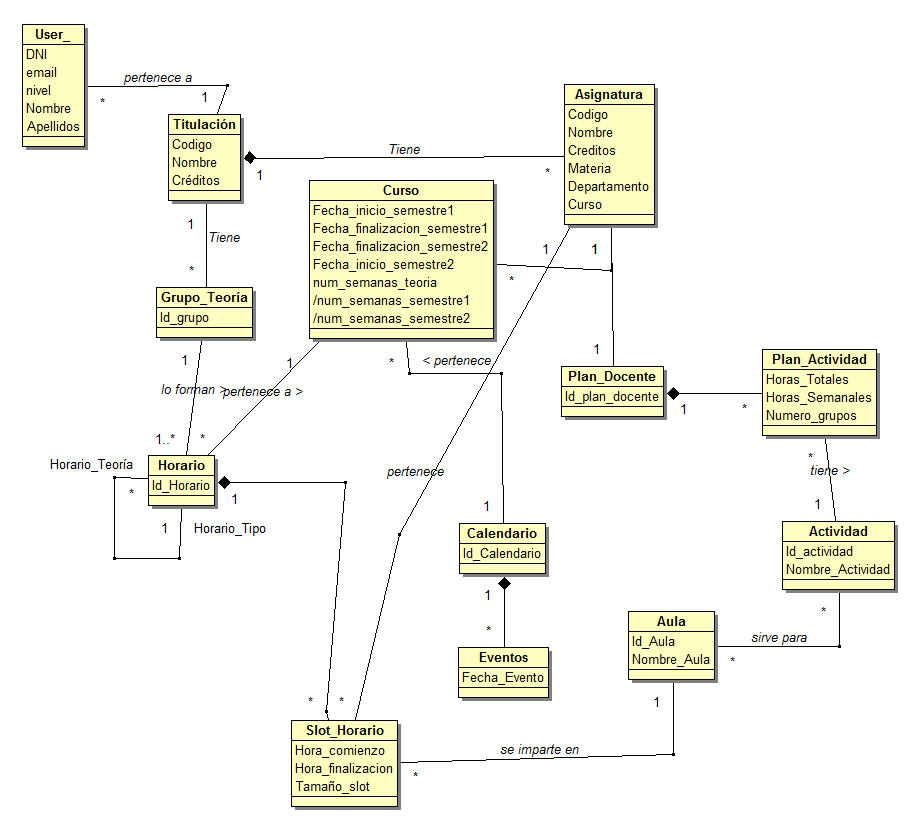
\includegraphics[scale=0.7]{./modeloconceptual.png}
  \end{center}
\caption{Diagrama del modelo conceptual de datos}
\end{figure}

\section{Modelo de comportamiento del sistema}

Para el modelo de comportamiento del sistema se mostrarán diferentes diagramas de secuencia del sistema. El diagrama define las interacciones entre actores y sistema, también se detallarán los contratos de las operaciones del sistema, para describir en detalle qué hace cada operación.
\paragraph{}
Al existir muchos casos de uso similares, sólo se detallarán los más relevantes de cada subsistema.

\subsection{Caso de uso: Registrar titulación}

\begin{figure}[H] 
  \label{comportamiento-reg-titulacion} 
	\begin{center}
    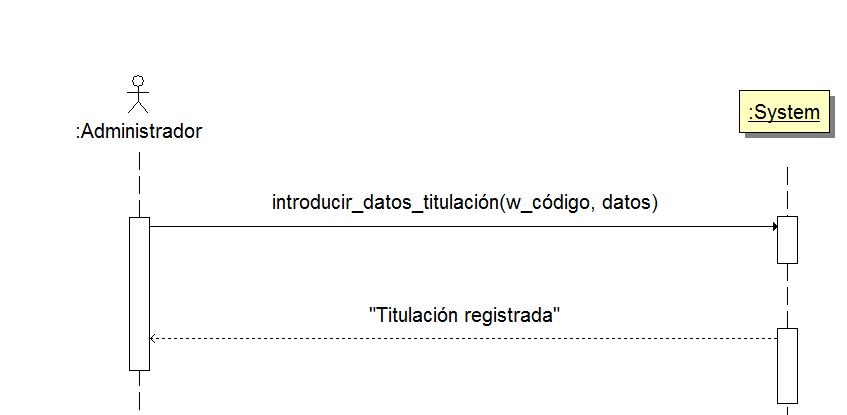
\includegraphics[scale=0.5]{./secuencia-reg-titulacion.png}
  \end{center}
\caption{Diagrama de secuencia del caso de uso Registrar titulación}
\end{figure}

\subsubsection{Contrato de la operación: introducir\_datos\_titulación}
\begin{itemize}
\item {\bf Responsabilidades:} Registrar una titulación en el sistema.
\item {\bf Referencias cruzadas:} Caso de uso {\em registrar titulación}, Caso de uso {\em editar titulación}.
\item {\bf Precondiciones:} No existe ninguna titulación con código = w\_código.
\item {\bf Postcondiciones:} Se crea una instancia T de Titulación. Se asignan w\_código y datos a T.
\end{itemize}

\subsection{Caso de uso: Registrar asignatura}

\begin{figure}[H] 
  \label{comportamiento-reg-asignatura} 
	\begin{center}
    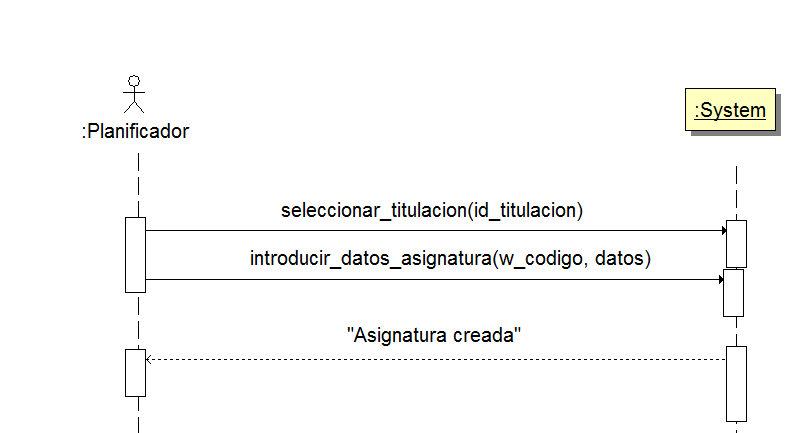
\includegraphics[scale=0.5]{./secuencia-reg-asignatura.png}
  \end{center}
\caption{Diagrama de secuencia del caso de uso Registrar asignatura}
\end{figure}

\subsubsection{Contrato de la operación: seleccionar\_titulacion}
\begin{itemize}
\item {\bf Responsabilidades:} Seleccionar una titulación para añadirle una asignatura.
\item {\bf Referencias cruzadas:} Caso de uso {\em registrar asignatura}, Caso de uso {\em editar asignatura}
\item {\bf Precondiciones:} Existe una titulación con t.id = id\_titulación.
\item {\bf Postcondiciones:} Se devuelve una instancia T de Titulación con T.id = id\_titulación.
\end{itemize}

\subsubsection{Contrato de la operación: introducir\_datos\_asignatura}
\begin{itemize}
\item {\bf Responsabilidades:} Registrar una asignatura y asociarla a una titulación.
\item {\bf Referencias cruzadas:} Caso de uso {\em registrar asignatura}, Caso de uso {\em editar asignatura}
\item {\bf Precondiciones:} No existe ninguna asignatura con código = w\_codigo.
\item {\bf Postcondiciones:} Se crea una instancia A de Asignatura. Se asigna A.codigo = w\_codigo y A.datos = datos.
\end{itemize}

\subsection{Caso de uso: Editar asignatura}
\begin{figure}[H] 
  \label{comportamiento-edit-asignatura} 
	\begin{center}
    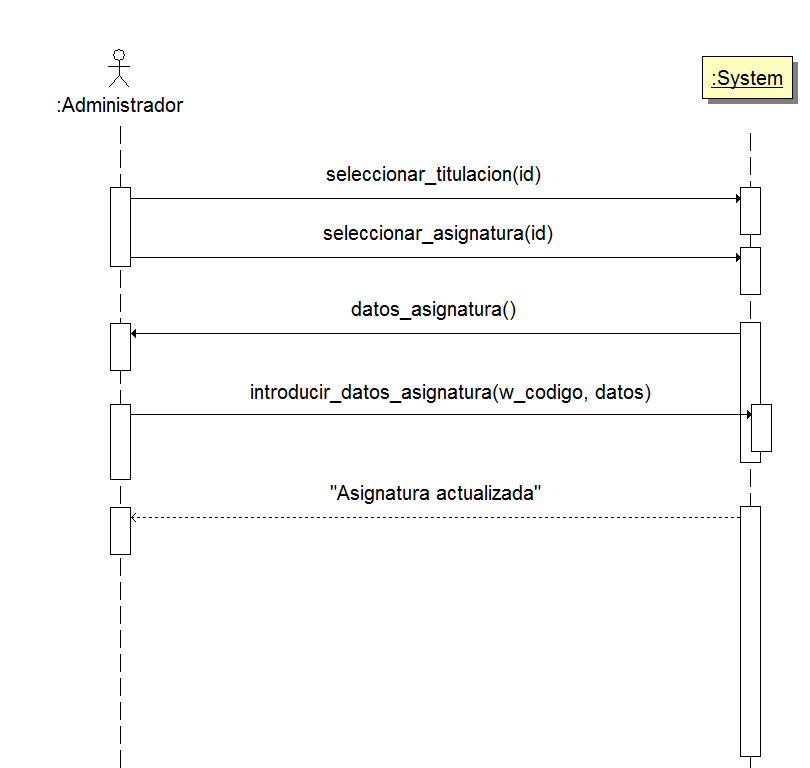
\includegraphics[scale=0.5]{./secuencia-edit-asignatura.png}
  \end{center}
\caption{Diagrama de secuencia del caso de uso Editar asignatura}
\end{figure}

\subsubsection{Contrato de la operación: seleccionar\_asignatura}
\begin{itemize}
\item {\bf Responsabilidades:} Devolver una instancia de Asignatura para poder editar sus datos.
\item {\bf Referencias cruzadas:} Caso de uso {\em editar asignatura}, Caso de uso {\em borrar asignatura}.
\item {\bf Precondiciones:} Debe existir una Asignatura registrada en el sistema con A.id = id\_asignatura.
\item {\bf Postcondiciones:} Se devuelve una instancia A de Asignatura con A.id = id\_asignatura.
\end{itemize}

\subsection{Caso de uso: Borrar asignatura}
\begin{figure}[H] 
  \label{comportamiento-borrar-asignatura} 
	\begin{center}
    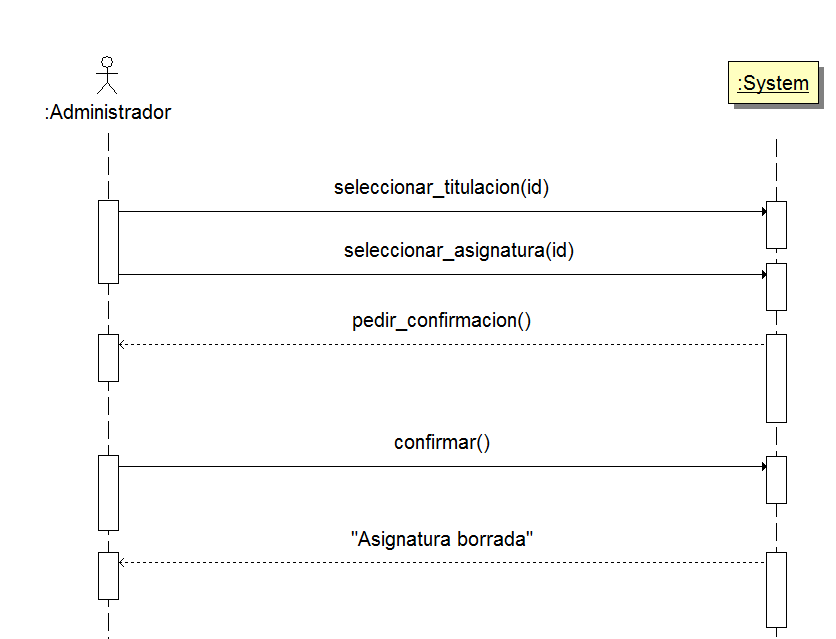
\includegraphics[scale=0.5]{./secuencia-borrar-asignatura.png}
  \end{center}
\caption{Diagrama de secuencia del caso de uso Borrar asignatura}
\end{figure}

\subsection{Caso de uso: Importar asignatura}
\begin{figure}[H] 
  \label{comportamiento-importar-asignatura} 
	\begin{center}
    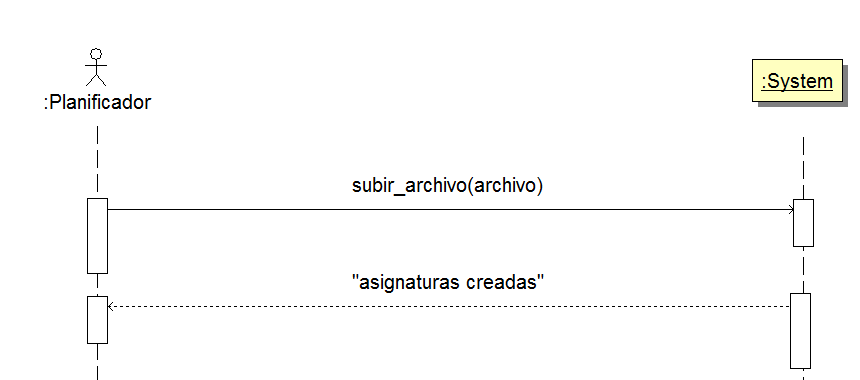
\includegraphics[scale=0.5]{./secuencia-importar-asignatura.png}
  \end{center}
\caption{Diagrama de secuencia del caso de uso Importar asignatura}
\end{figure}

\subsubsection{Contrato de la operación: subir\_archivo}
\begin{itemize}
\item {\bf Responsabilidades:} Crear asignaturas masivamente capturando la información de las líneas de un archivo.
\item {\bf Referencias cruzadas:} Caso de uso {\em importar asignatura}, Caso de uso {\em importar titulación}, Caso de uso {\em importar plan docente}.
\item {\bf Precondiciones:} Por cada línea del archivo, no existe una instancia de la clase a la que se pretende añadir información con la misma clave que aparece en la línea.
\item {\bf Postcondiciones:} Por cada línea se crea una instancia de la clase con id = id\_linea.
\end{itemize}

\subsection{Caso de uso: Crear plan docente}
\begin{figure}[H] 
  \label{comportamiento-crear-plandocente} 
	\begin{center}
    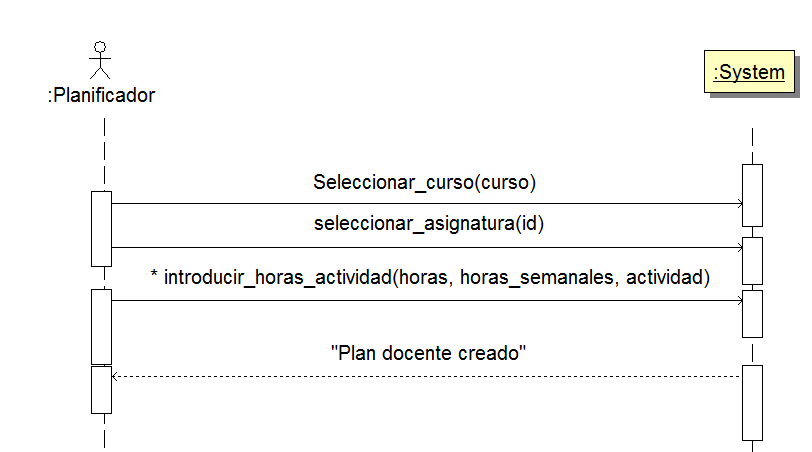
\includegraphics[scale=0.5]{./secuencia-crear-plandocente.png}
  \end{center}
\caption{Diagrama de secuencia del caso de uso Crear plan docente}
\end{figure}

\subsubsection{Contrato de la operación: introducir\_horas\_actividad}
\begin{itemize}
\item {\bf Responsabilidades:} Añadir la planificación docente de una actividad concreta al sistema.
\item {\bf Referencias cruzadas:} Caso de uso {\em crear plan docente}, Caso de uso {\em editar plan docente}
\item {\bf Precondiciones:} La actividad existe en el sistema.
\item {\bf Postcondiciones:} Se crea una instancia P de Plan\_Actividad con P.actividad = actividad, P.horas = horas y  P.horas\_semanales = horas\_semanales, además se asocia con la asignatura A.
\end{itemize}

\subsection{Caso de uso: Generar informe de asignatura}
\begin{figure}[H] 
  \label{comportamiento-generar-informe} 
	\begin{center}
    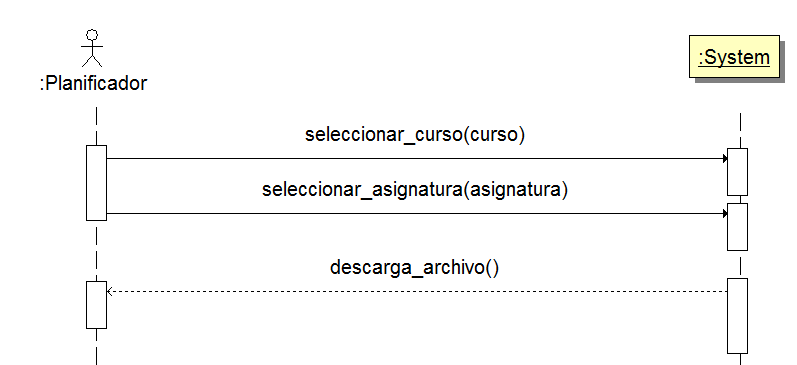
\includegraphics[scale=0.5]{./secuencia-gen-informe.png}
  \end{center}
\caption{Diagrama de secuencia del caso de uso Generar informe de asignatura}

\subsection{Caso de uso: Añadir evento al calendario}
\begin{figure}[H] 
  \label{comportamiento-anadir-evento} 
	\begin{center}
    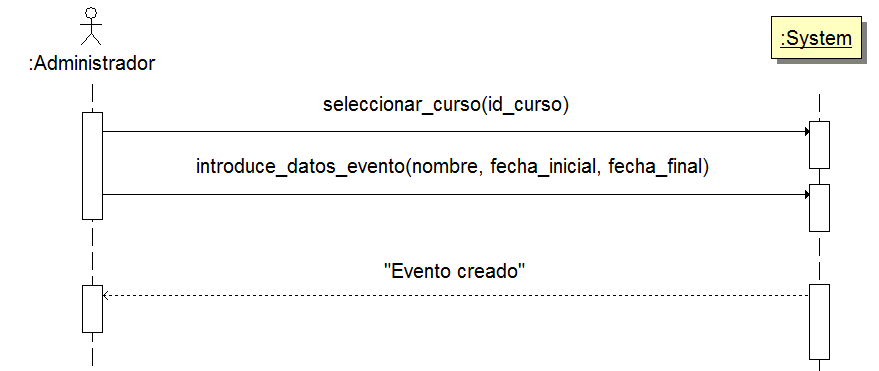
\includegraphics[scale=0.5]{./secuencia-crear-evento.png}
  \end{center}
\caption{Diagrama de secuencia del caso de uso Añadir evento al calendario}
\end{figure}
\end{figure}

\subsubsection{Contrato de la operación: seleccionar curso}
\begin{itemize}
\item {\bf Responsabilidades:} Seleccionar un curso para hacer operaciones con el o asociarlo con otras clases.
\item {\bf Referencias cruzadas:} Caso de uso {\em Añadir evento al calendario}.
\item {\bf Precondiciones:} Existe un curso C con C.id\_curso = id\_curso.
\item {\bf Postcondiciones:} Se devuelve una instancia C de curso.
\end{itemize}

\subsubsection{Contrato de la operación: introduce\_datos\_evento}
\begin{itemize}
\item {\bf Responsabilidades:} Crear un evento en el calendario del curso C.
\item {\bf Referencias cruzadas:} Caso de uso {\em Añadir evento al calendario}.
\item {\bf Precondiciones:} No existe ningún evento con fechas entre las introducidas.
\item {\bf Postcondiciones:} Se crea una instancia E de Evento con E.fecha\_inicial = fecha\_inicial, E.fecha\_final = fecha\_final y E.nombre = nombre y se asocia a C.
\end{itemize}

\subsection{Caso de uso: Exportar calendario}
\begin{figure}[H] 
  \label{comportamiento-exportar-calendario} 
	\begin{center}
    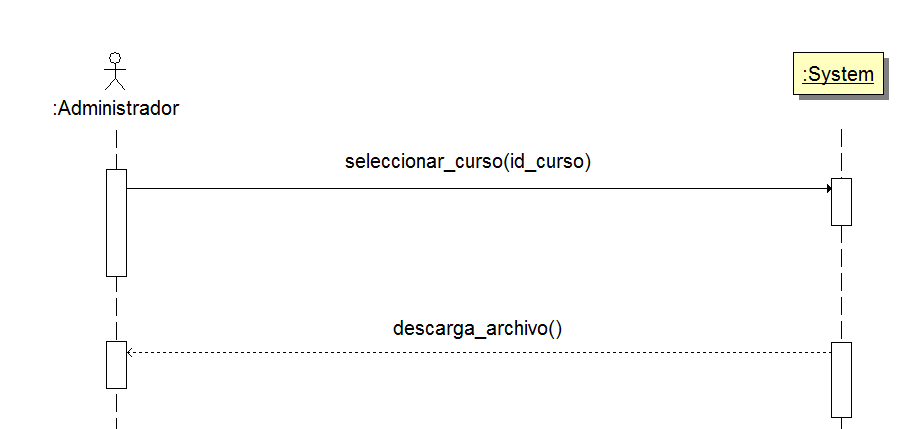
\includegraphics[scale=0.5]{./secuencia-exportar-calendario.png}
  \end{center}
\caption{Diagrama de secuencia del caso de uso Exportar calendario}
\end{figure}


\subsection{Caso de uso: Seleccionar grupos de teoría}
\begin{figure}[H] 
  \label{comportamiento-seleccionar-grupos} 
	\begin{center}
    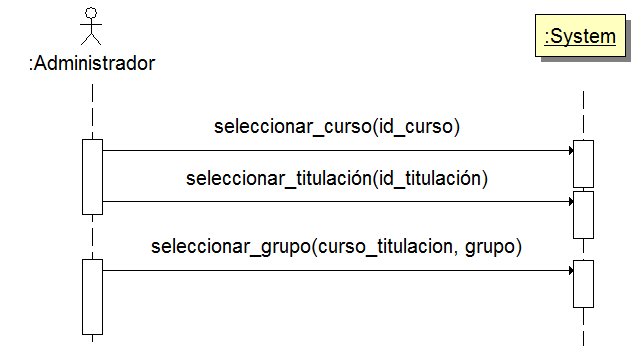
\includegraphics[scale=0.5]{./secuencia-seleccionar-grupo.png}
  \end{center}
\caption{Diagrama de secuencia del caso de uso Seleccionar grupos de teoría}
\end{figure}

\subsubsection{Contrato de la operación: seleccionar\_grupo}
\begin{itemize}
\item {\bf Responsabilidades:} Seleccionar un grupo de una titulación para hacer uso de él en otro caso de uso.
\item {\bf Referencias cruzadas:} Caso de uso {\em seleccionar grupos de teoría}
\item {\bf Precondiciones:} El curso indicado está dentro de los cursos de la titulación.
\\El grupo ha sido creado.
\item {\bf Postcondiciones:} Se devuelve una instancia G del Grupo.
\end{itemize}

\subsection{Caso de uso: Añadir grupo de teoría}
\begin{figure}[H] 
  \label{comportamiento-anadir-grupos} 
	\begin{center}
    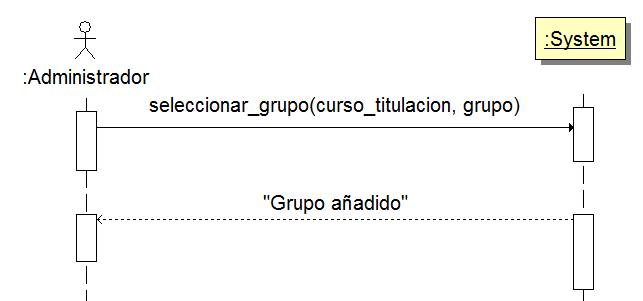
\includegraphics[scale=0.5]{./secuencia-anadir-grupo.png}
  \end{center}
\caption{Diagrama de secuencia del caso de uso Añadir grupo de teoría}
\end{figure}

\subsection{Caso de uso: Eliminar grupo de teoría}
\begin{figure}[H] 
  \label{comportamiento-borrar-grupos} 
	\begin{center}
    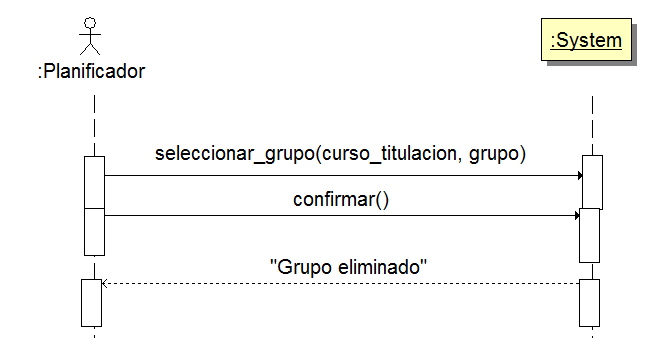
\includegraphics[scale=0.5]{./secuencia-borrar-grupo.png}
  \end{center}
\caption{Diagrama de secuencia del caso de uso Eliminar grupo de teoría}
\end{figure}

\subsection{Caso de uso: Ubicar slot de horario}
\begin{figure}[H] 
  \label{comportamiento-ubicar-slot} 
	\begin{center}
    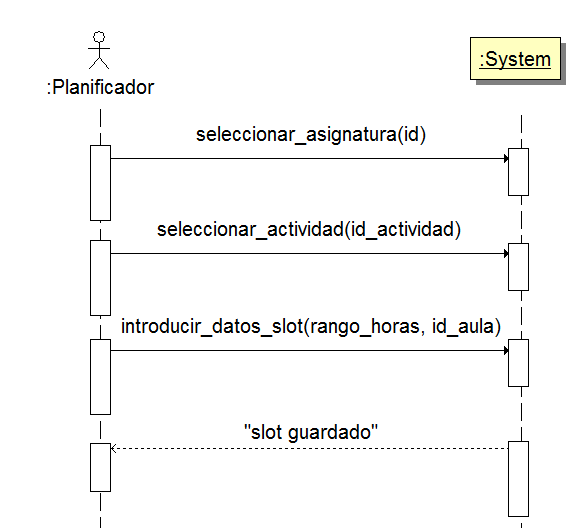
\includegraphics[scale=0.5]{./secuencia-ubicar-slot.png}
  \end{center}
\caption{Diagrama de secuencia del caso de uso Ubicar slot de horario}
\end{figure}

\subsubsection{Contrato de la operación: seleccionar\_actividad}
\begin{itemize}
\item {\bf Responsabilidades:} Seleccionar una actividad para introducirla en el horario
\item {\bf Referencias cruzadas:} Caso de uso {\em ubicar slot de horario}.
\item {\bf Precondiciones:} La asignatura elegida dispone de horas en el plan docente para esa actividad.
\item {\bf Postcondiciones:} Se devuelve una instancia de un Slot de horario para esa asignatura y actividad.
\end{itemize}

\subsubsection{Contrato de la operación: introducir\_datos\_slot}
\begin{itemize}
\item {\bf Responsabilidades:} Ubicar en el horario un slot de una actividad de una asignatura.
\item {\bf Referencias cruzadas:} Caso de uso {\em ubicar slot de horario}
\item {\bf Precondiciones:} Si el slot es de teoría no se solapa con otro slot. No se debe solapar con otro slot con el mismo id\_aula.
\item {\bf Postcondiciones:} El slot queda ubicado en el horario.
\end{itemize}

\subsection{Caso de uso: Editar horario tipo}
\begin{figure}[H] 
  \label{comportamiento-editar-tipo} 
	\begin{center}
    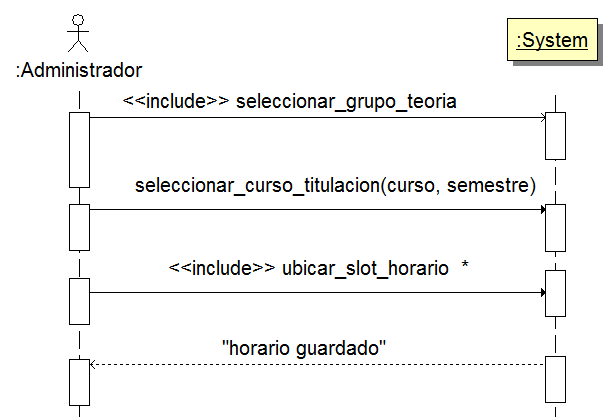
\includegraphics[scale=0.5]{./secuencia-editar-tipo.png}
  \end{center}
\caption{Diagrama de secuencia del caso de uso Editar horario tipo}
\end{figure}

\subsubsection{Contrato de la operación: seleccionar\_curso\_titulacion}
\begin{itemize}
\item {\bf Responsabilidades:} Seleccionar una instancia del Horario
\item {\bf Referencias cruzadas:} Caso de uso {\em editar horario tipo}, Caso de uso {\em editar horario semana inicial}.
\item {\bf Precondiciones:} El curso está dentro de los que tiene la titulación.
\item {\bf Postcondiciones:} Se devuelve una instancia de Horario (o se crea una si no existe).
\end{itemize}

\subsection{Caso de uso: Comprobar grupo de teoría}
\begin{figure}[H] 
  \label{comportamiento-comprobar-grupo} 
	\begin{center}
    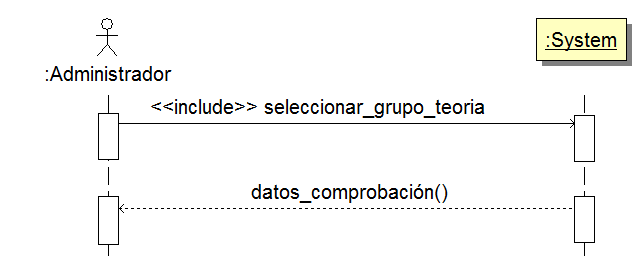
\includegraphics[scale=0.5]{./secuencia-comprobar-grupo.png}
  \end{center}
\caption{Diagrama de secuencia del caso de uso Comprobar grupo de teoría}
\end{figure}

\subsection{Caso de uso: Crear aula}

\begin{figure}[H] 
  \label{comportamiento-crear-aula} 
	\begin{center}
    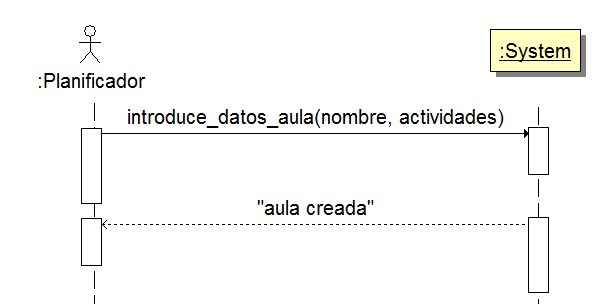
\includegraphics[scale=0.5]{./secuencia-crear-aula.png}
  \end{center}
\caption{Diagrama de secuencia del caso de uso Crear aula}
\end{figure}

\subsubsection{Contrato de la operación: introducir\_datos\_aula}
\begin{itemize}
\item {\bf Responsabilidades:} Crear un aula en el sistema.
\item {\bf Referencias cruzadas:} Caso de uso {\em crear aula}, Caso de uso {\em Editar aula}.
\item {\bf Precondiciones:} No existe ningún aula en el sistema con A.nombre = nombre.
\item {\bf Postcondiciones:} Se crea una instancia A de Aula con A.nombre = nombre y A.actividades = actividades.
\end{itemize}

\subsection{Caso de uso: Borrar aula}
\begin{figure}[H] 
  \label{comportamiento-borrar-aula} 
	\begin{center}
    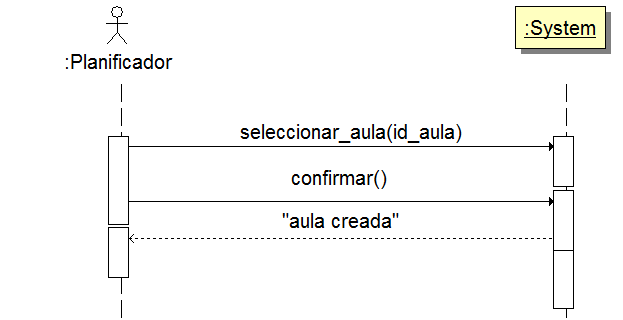
\includegraphics[scale=0.5]{./secuencia-borrar-aula.png}
  \end{center}
\caption{Diagrama de secuencia del caso de uso Borrar aula}
\end{figure}

\subsubsection{Contrato de la operación: seleccionar\_aula}
\begin{itemize}
\item {\bf Responsabilidades:} Seleccionar un aula para borrarla o editarla.
\item {\bf Referencias cruzadas:} Caso de uso {\em borrar aula}, Caso de uso {\em editar aula}.
\item {\bf Precondiciones:} Existe un aula en el sistema con A.id\_aula = id\_aula.
\item {\bf Postcondiciones:} Se devuelve una instancia A de aula con A.id\_aula = id\_aula.
\end{itemize}

\subsection{Caso de uso: Editar aula}
\begin{figure}[H] 
  \label{comportamiento-editar-aula} 
	\begin{center}
    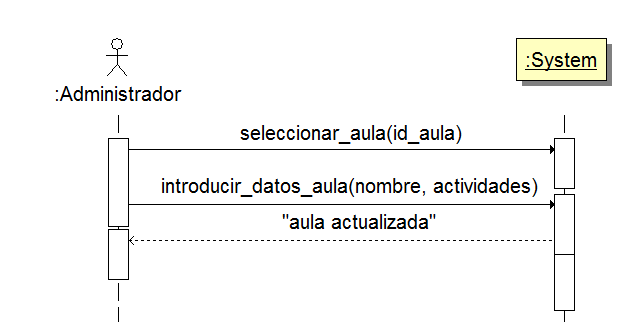
\includegraphics[scale=0.5]{./secuencia-editar-aula.png}
  \end{center}
\caption{Diagrama de secuencia del caso de uso Editar aula}
\end{figure}
% Plantilla para contratos de operaciones


\backmatter % Apéndices, bibliografia ...


\clearpage
\addcontentsline{toc}{chapter}{Bibliografia y referencias}
\bibliographystyle{plain}
\bibliography{bibliografia}


\addcontentsline{toc}{chapter}{Software usado}
\chapter*{Software utilizado}
% -*-programas.tex-*-
% Este fichero es parte de la plantilla LaTeX para
% la realización de Proyectos Final de Carrera, protejido
% bajo los términos de la licencia GFDL.
% Para más información, la licencia completa viene incluida en el
% fichero fdl-1.3.tex

% Copyright (C) 2009 Pablo Recio Quijano 
Es usual en un PFC referenciar que software has usado para la
realización del mismo. Aprovecharé este apartado para que conozcas
alguna herramienta que puede serte de ayuda para realizar tus
documentos en \LaTeX{}

\section*{Emacs + Auc\TeX}

Emacs es uno de los programas de edición más usados por
desarrolladores de software, ya que es bastante versatil admitiendo
gran cantidad de ``plugins'' o extensiones que permiten ampliar aun
más sus funcionalidades.\\

Uno de estos plugins es Auc\TeX \cite{pdf:auctex}, el cual incluye
rutas para ciertos comandos, resaltado de sintaxis, previsualización
del documento, menú matemático en el cual podemos acceder e insertar
la gran mayoria de los símbolos matemáticos, para no tener que
memorizarlos. Podemos ver un ejemplo de Emacs + Auc\TeX en la figura
\ref{auctex}

\figura{Auctex.png}{scale=0.6}{Emacs + Auc\TeX}{auctex}{h}

Por ejemplo, para cerrar un entorno $\backslash$\texttt{begin()}, con su
respectivo $\backslash$\texttt{end()}, utilizaremos el atajo
\comando{C-c M-]}, para añadir un $\backslash$\texttt{item}, tenemos
el atajo \comando{C-c C-j}, y así unos cuantos, que una vez que nos
habituamos a ellos, son bastante cómodos.\\

Además, es bastante configurable, con indentado automático, corrector
ortográfico y demás. El fichero adjunto a este documento,
\emph{conf\_emacs} incluye una configuración con varias de estas
opciones.

\section*{Doxygen}

Realmente, \programa{Doxygen} \cite{website:doxygen} no es una herramienta
que vayamos a utilizar para realizar documentos \LaTeX{}
directmaente. Sin embargo, para la documentación de código si es
bastante util.\\

Esta herramienta realiza una documentación automática de código
fuente. Es decir, para nuestro PFC, podemos utilizar para generar la
documentación de las APIs de nuestras librerias y demás. Puede generar
esta documentación en varios formatos, y entre ellos, \LaTeX, de forma
que podemos utilizar ese código generado en nuestra memoria de forma
automática.

\section*{GNU Make}

\programa{GNU Make} es el programa de recompilación y de control de
dependencias por excelencia. Se puede utilizar para compilar proyectos
software en diversos códigos, o como en el caso de este documento,
para compilar documentos \LaTeX{} con diversas opciones.\\

Para más información \cite{pdf:make}

\section*{Dia}

\programa{Dia} es un editor de gráficos vectoriales el cual incluye
distintas plantillas para distintos tipos de gráficos, como pueden ser
UML, ERe, diagramas de flujo, esquemas Cisco de red y un larguísimo
etcétera. Podemos ver el interfaz en la figura \ref{dia}

\figura{dia.png}{scale=0.6}{Interfaz de Dia}{dia}{h}

Estos diagramas podemos exportarlos a diversos formatos de imagen
(\texttt{.png}, \texttt{.eps}, ...) o a formato \texttt{.tex}, como
vimos anteriormente.

\addcontentsline{toc}{chapter}{Instalación de \LaTeX}
\chapter*{Instalación de \LaTeX}
\section{Prerrequisitos}

Para poder instalar la aplicación en un servidor debemos tener previamente instalados una serie de programas, disponibles tanto en Linux como en Windows. A continuación se enumeran estos paquetes necesarios para el funcionamiento:

\begin{itemize}

\item {\bf MySQL Server}: Es el sistema gestor de base de datos de la aplicación. En Linux se puede obtener de los repositorios, también se puede descargar de la página oficial:\\
\href{http://dev.mysql.com/downloads/mysql/}{http://dev.mysql.com/downloads/mysql/}\\
Es importante conocer la contraseña de root ya que será necesaria para crear la base de datos y el usuario al que será asociada la aplicación.
\item {\bf PHP}: Debemos tener instalada una versión de PHP igual o superior a la 5.3, se puede descargar sin problemas de los repositorios, o bien de la página oficial.
\item {\bf Apache httpd server}: También disponible tanto en la página oficial como en los repositorios.
\end{itemize}

\section{Instalación de la aplicación}
La aplicación se proporciona en un fichero .zip, así que solo habrá que descomprimirlo en una carpeta del servidor web, es importante saber la ruta desde la que se accede en el servidor, ya que habrá que configurar la aplicación apropiadamente más adelante.
\paragraph{}
Es importante no cambiar ningún fichero ni carpeta en la jerarquía de directorios de la aplicación, sino el funcionamiento podría alterarse. También es importante no borrar el fichero .htaccess disponible en la raíz de la aplicación.

\section{Puesta en funcionamiento}
Para que la aplicación funcione, necesita tener una base de datos creada, además del usuario con el que se conectará desde la aplicación. Para ello se deben seguir los pasos descritos a continuación:
\begin{itemize}
\item Lo primero que hay que hacer es acceder a {\em MySQL} con el usuario root, escribiendo desde el terminal lo siguiente:
\begin{lstlisting}[style=consola]
	mysql -u root -p
\end{lstlisting}
Y a continuación se nos pedirá la contraseña.
\item El siguiente paso es crear la base de datos con el nombre ''gestiongrados'', para ello escribimos:
\begin{lstlisting}[style=consola]
	mysql > CREATE DATABASE gestiongrados;
\end{lstlisting}
\item Una vez creada la base de datos, hay que crear el usuario ''gestiongrados'', escribimos lo siguiente en la consola de {\em MySQL}:
\begin{lstlisting}[style=consola]
	mysql > GRANT CREATE, SELECT, INSERT, DELETE, UPDATE 
	ON gestiongrados.* to 'gestiongrados'@'localhost' 
	IDENTIFIED BY 'ges1234';
\end{lstlisting}
Nótese que se ha asignado el password ges1234, puede ser cambiado, pero deberá ser configurado en la aplicación más adelante.
\item Aplicamos los cambios en la base de datos:
\begin{lstlisting}[style=consola]
	mysql > FLUSH PRIVILEGES
\end{lstlisting}
\end{itemize}

Ya tenemos la base de datos creada, pero ahora hay que modificar algunos parámetros de configuración en el fichero de configuración de la aplicación. Para ello abrimos el fichero './application/config/config.php'.\\
Este fichero únicamente hace asignaciones en un array asociativo \$config, donde cada clave es un parámetro de configuración. Debemos hacer la siguiente modificación:

\begin{itemize}
\item En primer lugar debemos modificar el valor de la clave ''base\_url'', que es el que contiene la url y ruta de la carpeta del servidor donde se ubica la aplicación, por ejemplo si el servidor es gestion.uca.es, y la ruta es /gestiongrados, el valor de la clave deberá ser:
\begin{lstlisting}[style=PHP]
$config['base_url'] = 'http://gestion.uca.es/gestiongrados';
\end{lstlisting}
\item No modificar ningún otro parámetro, ya que esto podría provocar un mal funcionamiento de la aplicación.
\end{itemize}

A continuación debemos ir al fichero './application/config/database.php' y hacer las siguientes modificaciones:
\begin{itemize}
\item Modificar el valor del hostname, que corresponderá al servidor donde estará ubicada la base de datos.
\begin{lstlisting}[style=PHP]
	$db['default']['hostname'] = 'localhost';
\end{lstlisting}
\item Modificar el nombre de usuario si se ha cambiado al crear la base de datos, sino dejar el que está ('gestiongrados'):
\begin{lstlisting}[style=PHP]
	$db['default']['username'] = 'gestiongrados';
\end{lstlisting}
\item Modificar el password si se ha modificado al crear el usuario en la base de datos, sino dejar el que está ('ges1234'):
\begin{lstlisting}[style=PHP]
	$db['default']['password'] = 'ges1234';
\end{lstlisting}
\item Modificar el nombre de la base de datos si se ha modificado al crearla, sino dejar el que está ('gestiongrados'):
\begin{lstlisting}[style=PHP]
	$db['default']['database'] = 'gestiongrados';
\end{lstlisting}
\item Dejar todos los demás parámetros tal cual están, sino se podría obtener un mal funcionamiento.
\end{itemize}

Una vez hecho esto, podremos finalizar la aplicación entrando en la ruta de instalación de la aplicación, que se encargará de crear la estructura de la base de datos además de un usuario administrador, al que podremos asignar una contraseña, para ello debemos escribir en el navegador la ruta base de la aplicación, seguido de "/install", pantalla en la que se nos pedirá una contraseña para finalizar la instalación de la aplicación, además de una dirección de correo electrónico que será la que se use para entrar en la aplicación. Una vez terminada la instalación, se nos indicará con un mensaje, y podremos empezar a trabajar con ella.



% This is set up to run with pdflatex.
%---------The file header---------------------------------------------
%---------------------------------------------------------------------
\chapter*{\rlap{GNU Free Documentation License}}
\phantomsection  % so hyperref creates bookmarks
\addcontentsline{toc}{chapter}{GNU Free Documentation License}
%\label{label_fdl}

 \begin{center}

       Version 1.3, 3 November 2008


 Copyright \copyright{} 2000, 2001, 2002, 2007, 2008  Free Software Foundation, Inc.
 
 \bigskip
 
     <http://fsf.org/>
  
 \bigskip
 
 Everyone is permitted to copy and distribute verbatim copies
 of this license document, but changing it is not allowed.
\end{center}


\begin{center}
{\bf\large Preamble}
\end{center}

The purpose of this License is to make a manual, textbook, or other
functional and useful document ``free'' in the sense of freedom: to
assure everyone the effective freedom to copy and redistribute it,
with or without modifying it, either commercially or noncommercially.
Secondarily, this License preserves for the author and publisher a way
to get credit for their work, while not being considered responsible
for modifications made by others.

This License is a kind of ``copyleft'', which means that derivative
works of the document must themselves be free in the same sense.  It
complements the GNU General Public License, which is a copyleft
license designed for free software.

We have designed this License in order to use it for manuals for free
software, because free software needs free documentation: a free
program should come with manuals providing the same freedoms that the
software does.  But this License is not limited to software manuals;
it can be used for any textual work, regardless of subject matter or
whether it is published as a printed book.  We recommend this License
principally for works whose purpose is instruction or reference.


\begin{center}
{\Large\bf 1. APPLICABILITY AND DEFINITIONS\par}
\phantomsection
\addcontentsline{toc}{section}{1. APPLICABILITY AND DEFINITIONS}
\end{center}

This License applies to any manual or other work, in any medium, that
contains a notice placed by the copyright holder saying it can be
distributed under the terms of this License.  Such a notice grants a
world-wide, royalty-free license, unlimited in duration, to use that
work under the conditions stated herein.  The ``\textbf{Document}'', below,
refers to any such manual or work.  Any member of the public is a
licensee, and is addressed as ``\textbf{you}''.  You accept the license if you
copy, modify or distribute the work in a way requiring permission
under copyright law.

A ``\textbf{Modified Version}'' of the Document means any work containing the
Document or a portion of it, either copied verbatim, or with
modifications and/or translated into another language.

A ``\textbf{Secondary Section}'' is a named appendix or a front-matter section of
the Document that deals exclusively with the relationship of the
publishers or authors of the Document to the Document's overall subject
(or to related matters) and contains nothing that could fall directly
within that overall subject.  (Thus, if the Document is in part a
textbook of mathematics, a Secondary Section may not explain any
mathematics.)  The relationship could be a matter of historical
connection with the subject or with related matters, or of legal,
commercial, philosophical, ethical or political position regarding
them.

The ``\textbf{Invariant Sections}'' are certain Secondary Sections whose titles
are designated, as being those of Invariant Sections, in the notice
that says that the Document is released under this License.  If a
section does not fit the above definition of Secondary then it is not
allowed to be designated as Invariant.  The Document may contain zero
Invariant Sections.  If the Document does not identify any Invariant
Sections then there are none.

The ``\textbf{Cover Texts}'' are certain short passages of text that are listed,
as Front-Cover Texts or Back-Cover Texts, in the notice that says that
the Document is released under this License.  A Front-Cover Text may
be at most 5 words, and a Back-Cover Text may be at most 25 words.

A ``\textbf{Transparent}'' copy of the Document means a machine-readable copy,
represented in a format whose specification is available to the
general public, that is suitable for revising the document
straightforwardly with generic text editors or (for images composed of
pixels) generic paint programs or (for drawings) some widely available
drawing editor, and that is suitable for input to text formatters or
for automatic translation to a variety of formats suitable for input
to text formatters.  A copy made in an otherwise Transparent file
format whose markup, or absence of markup, has been arranged to thwart
or discourage subsequent modification by readers is not Transparent.
An image format is not Transparent if used for any substantial amount
of text.  A copy that is not ``Transparent'' is called ``\textbf{Opaque}''.

Examples of suitable formats for Transparent copies include plain
ASCII without markup, Texinfo input format, LaTeX input format, SGML
or XML using a publicly available DTD, and standard-conforming simple
HTML, PostScript or PDF designed for human modification.  Examples of
transparent image formats include PNG, XCF and JPG.  Opaque formats
include proprietary formats that can be read and edited only by
proprietary word processors, SGML or XML for which the DTD and/or
processing tools are not generally available, and the
machine-generated HTML, PostScript or PDF produced by some word
processors for output purposes only.

The ``\textbf{Title Page}'' means, for a printed book, the title page itself,
plus such following pages as are needed to hold, legibly, the material
this License requires to appear in the title page.  For works in
formats which do not have any title page as such, ``Title Page'' means
the text near the most prominent appearance of the work's title,
preceding the beginning of the body of the text.

The ``\textbf{publisher}'' means any person or entity that distributes
copies of the Document to the public.

A section ``\textbf{Entitled XYZ}'' means a named subunit of the Document whose
title either is precisely XYZ or contains XYZ in parentheses following
text that translates XYZ in another language.  (Here XYZ stands for a
specific section name mentioned below, such as ``\textbf{Acknowledgements}'',
``\textbf{Dedications}'', ``\textbf{Endorsements}'', or ``\textbf{History}''.)  
To ``\textbf{Preserve the Title}''
of such a section when you modify the Document means that it remains a
section ``Entitled XYZ'' according to this definition.

The Document may include Warranty Disclaimers next to the notice which
states that this License applies to the Document.  These Warranty
Disclaimers are considered to be included by reference in this
License, but only as regards disclaiming warranties: any other
implication that these Warranty Disclaimers may have is void and has
no effect on the meaning of this License.


\begin{center}
{\Large\bf 2. VERBATIM COPYING\par}
\phantomsection
\addcontentsline{toc}{section}{2. VERBATIM COPYING}
\end{center}

You may copy and distribute the Document in any medium, either
commercially or noncommercially, provided that this License, the
copyright notices, and the license notice saying this License applies
to the Document are reproduced in all copies, and that you add no other
conditions whatsoever to those of this License.  You may not use
technical measures to obstruct or control the reading or further
copying of the copies you make or distribute.  However, you may accept
compensation in exchange for copies.  If you distribute a large enough
number of copies you must also follow the conditions in section~3.

You may also lend copies, under the same conditions stated above, and
you may publicly display copies.


\begin{center}
{\Large\bf 3. COPYING IN QUANTITY\par}
\phantomsection
\addcontentsline{toc}{section}{3. COPYING IN QUANTITY}
\end{center}


If you publish printed copies (or copies in media that commonly have
printed covers) of the Document, numbering more than 100, and the
Document's license notice requires Cover Texts, you must enclose the
copies in covers that carry, clearly and legibly, all these Cover
Texts: Front-Cover Texts on the front cover, and Back-Cover Texts on
the back cover.  Both covers must also clearly and legibly identify
you as the publisher of these copies.  The front cover must present
the full title with all words of the title equally prominent and
visible.  You may add other material on the covers in addition.
Copying with changes limited to the covers, as long as they preserve
the title of the Document and satisfy these conditions, can be treated
as verbatim copying in other respects.

If the required texts for either cover are too voluminous to fit
legibly, you should put the first ones listed (as many as fit
reasonably) on the actual cover, and continue the rest onto adjacent
pages.

If you publish or distribute Opaque copies of the Document numbering
more than 100, you must either include a machine-readable Transparent
copy along with each Opaque copy, or state in or with each Opaque copy
a computer-network location from which the general network-using
public has access to download using public-standard network protocols
a complete Transparent copy of the Document, free of added material.
If you use the latter option, you must take reasonably prudent steps,
when you begin distribution of Opaque copies in quantity, to ensure
that this Transparent copy will remain thus accessible at the stated
location until at least one year after the last time you distribute an
Opaque copy (directly or through your agents or retailers) of that
edition to the public.

It is requested, but not required, that you contact the authors of the
Document well before redistributing any large number of copies, to give
them a chance to provide you with an updated version of the Document.


\begin{center}
{\Large\bf 4. MODIFICATIONS\par}
\phantomsection
\addcontentsline{toc}{section}{4. MODIFICATIONS}
\end{center}

You may copy and distribute a Modified Version of the Document under
the conditions of sections 2 and 3 above, provided that you release
the Modified Version under precisely this License, with the Modified
Version filling the role of the Document, thus licensing distribution
and modification of the Modified Version to whoever possesses a copy
of it.  In addition, you must do these things in the Modified Version:

\begin{itemize}
\item[A.] 
   Use in the Title Page (and on the covers, if any) a title distinct
   from that of the Document, and from those of previous versions
   (which should, if there were any, be listed in the History section
   of the Document).  You may use the same title as a previous version
   if the original publisher of that version gives permission.
   
\item[B.]
   List on the Title Page, as authors, one or more persons or entities
   responsible for authorship of the modifications in the Modified
   Version, together with at least five of the principal authors of the
   Document (all of its principal authors, if it has fewer than five),
   unless they release you from this requirement.
   
\item[C.]
   State on the Title page the name of the publisher of the
   Modified Version, as the publisher.
   
\item[D.]
   Preserve all the copyright notices of the Document.
   
\item[E.]
   Add an appropriate copyright notice for your modifications
   adjacent to the other copyright notices.
   
\item[F.]
   Include, immediately after the copyright notices, a license notice
   giving the public permission to use the Modified Version under the
   terms of this License, in the form shown in the Addendum below.
   
\item[G.]
   Preserve in that license notice the full lists of Invariant Sections
   and required Cover Texts given in the Document's license notice.
   
\item[H.]
   Include an unaltered copy of this License.
   
\item[I.]
   Preserve the section Entitled ``History'', Preserve its Title, and add
   to it an item stating at least the title, year, new authors, and
   publisher of the Modified Version as given on the Title Page.  If
   there is no section Entitled ``History'' in the Document, create one
   stating the title, year, authors, and publisher of the Document as
   given on its Title Page, then add an item describing the Modified
   Version as stated in the previous sentence.
   
\item[J.]
   Preserve the network location, if any, given in the Document for
   public access to a Transparent copy of the Document, and likewise
   the network locations given in the Document for previous versions
   it was based on.  These may be placed in the ``History'' section.
   You may omit a network location for a work that was published at
   least four years before the Document itself, or if the original
   publisher of the version it refers to gives permission.
   
\item[K.]
   For any section Entitled ``Acknowledgements'' or ``Dedications'',
   Preserve the Title of the section, and preserve in the section all
   the substance and tone of each of the contributor acknowledgements
   and/or dedications given therein.
   
\item[L.]
   Preserve all the Invariant Sections of the Document,
   unaltered in their text and in their titles.  Section numbers
   or the equivalent are not considered part of the section titles.
   
\item[M.]
   Delete any section Entitled ``Endorsements''.  Such a section
   may not be included in the Modified Version.
   
\item[N.]
   Do not retitle any existing section to be Entitled ``Endorsements''
   or to conflict in title with any Invariant Section.
   
\item[O.]
   Preserve any Warranty Disclaimers.
\end{itemize}

If the Modified Version includes new front-matter sections or
appendices that qualify as Secondary Sections and contain no material
copied from the Document, you may at your option designate some or all
of these sections as invariant.  To do this, add their titles to the
list of Invariant Sections in the Modified Version's license notice.
These titles must be distinct from any other section titles.

You may add a section Entitled ``Endorsements'', provided it contains
nothing but endorsements of your Modified Version by various
parties---for example, statements of peer review or that the text has
been approved by an organization as the authoritative definition of a
standard.

You may add a passage of up to five words as a Front-Cover Text, and a
passage of up to 25 words as a Back-Cover Text, to the end of the list
of Cover Texts in the Modified Version.  Only one passage of
Front-Cover Text and one of Back-Cover Text may be added by (or
through arrangements made by) any one entity.  If the Document already
includes a cover text for the same cover, previously added by you or
by arrangement made by the same entity you are acting on behalf of,
you may not add another; but you may replace the old one, on explicit
permission from the previous publisher that added the old one.

The author(s) and publisher(s) of the Document do not by this License
give permission to use their names for publicity for or to assert or
imply endorsement of any Modified Version.


\begin{center}
{\Large\bf 5. COMBINING DOCUMENTS\par}
\phantomsection
\addcontentsline{toc}{section}{5. COMBINING DOCUMENTS}
\end{center}


You may combine the Document with other documents released under this
License, under the terms defined in section~4 above for modified
versions, provided that you include in the combination all of the
Invariant Sections of all of the original documents, unmodified, and
list them all as Invariant Sections of your combined work in its
license notice, and that you preserve all their Warranty Disclaimers.

The combined work need only contain one copy of this License, and
multiple identical Invariant Sections may be replaced with a single
copy.  If there are multiple Invariant Sections with the same name but
different contents, make the title of each such section unique by
adding at the end of it, in parentheses, the name of the original
author or publisher of that section if known, or else a unique number.
Make the same adjustment to the section titles in the list of
Invariant Sections in the license notice of the combined work.

In the combination, you must combine any sections Entitled ``History''
in the various original documents, forming one section Entitled
``History''; likewise combine any sections Entitled ``Acknowledgements'',
and any sections Entitled ``Dedications''.  You must delete all sections
Entitled ``Endorsements''.

\begin{center}
{\Large\bf 6. COLLECTIONS OF DOCUMENTS\par}
\phantomsection
\addcontentsline{toc}{section}{6. COLLECTIONS OF DOCUMENTS}
\end{center}

You may make a collection consisting of the Document and other documents
released under this License, and replace the individual copies of this
License in the various documents with a single copy that is included in
the collection, provided that you follow the rules of this License for
verbatim copying of each of the documents in all other respects.

You may extract a single document from such a collection, and distribute
it individually under this License, provided you insert a copy of this
License into the extracted document, and follow this License in all
other respects regarding verbatim copying of that document.


\begin{center}
{\Large\bf 7. AGGREGATION WITH INDEPENDENT WORKS\par}
\phantomsection
\addcontentsline{toc}{section}{7. AGGREGATION WITH INDEPENDENT WORKS}
\end{center}


A compilation of the Document or its derivatives with other separate
and independent documents or works, in or on a volume of a storage or
distribution medium, is called an ``aggregate'' if the copyright
resulting from the compilation is not used to limit the legal rights
of the compilation's users beyond what the individual works permit.
When the Document is included in an aggregate, this License does not
apply to the other works in the aggregate which are not themselves
derivative works of the Document.

If the Cover Text requirement of section~3 is applicable to these
copies of the Document, then if the Document is less than one half of
the entire aggregate, the Document's Cover Texts may be placed on
covers that bracket the Document within the aggregate, or the
electronic equivalent of covers if the Document is in electronic form.
Otherwise they must appear on printed covers that bracket the whole
aggregate.


\begin{center}
{\Large\bf 8. TRANSLATION\par}
\phantomsection
\addcontentsline{toc}{section}{8. TRANSLATION}
\end{center}


Translation is considered a kind of modification, so you may
distribute translations of the Document under the terms of section~4.
Replacing Invariant Sections with translations requires special
permission from their copyright holders, but you may include
translations of some or all Invariant Sections in addition to the
original versions of these Invariant Sections.  You may include a
translation of this License, and all the license notices in the
Document, and any Warranty Disclaimers, provided that you also include
the original English version of this License and the original versions
of those notices and disclaimers.  In case of a disagreement between
the translation and the original version of this License or a notice
or disclaimer, the original version will prevail.

If a section in the Document is Entitled ``Acknowledgements'',
``Dedications'', or ``History'', the requirement (section~4) to Preserve
its Title (section~1) will typically require changing the actual
title.


\begin{center}
{\Large\bf 9. TERMINATION\par}
\phantomsection
\addcontentsline{toc}{section}{9. TERMINATION}
\end{center}


You may not copy, modify, sublicense, or distribute the Document
except as expressly provided under this License.  Any attempt
otherwise to copy, modify, sublicense, or distribute it is void, and
will automatically terminate your rights under this License.

However, if you cease all violation of this License, then your license
from a particular copyright holder is reinstated (a) provisionally,
unless and until the copyright holder explicitly and finally
terminates your license, and (b) permanently, if the copyright holder
fails to notify you of the violation by some reasonable means prior to
60 days after the cessation.

Moreover, your license from a particular copyright holder is
reinstated permanently if the copyright holder notifies you of the
violation by some reasonable means, this is the first time you have
received notice of violation of this License (for any work) from that
copyright holder, and you cure the violation prior to 30 days after
your receipt of the notice.

Termination of your rights under this section does not terminate the
licenses of parties who have received copies or rights from you under
this License.  If your rights have been terminated and not permanently
reinstated, receipt of a copy of some or all of the same material does
not give you any rights to use it.


\begin{center}
{\Large\bf 10. FUTURE REVISIONS OF THIS LICENSE\par}
\phantomsection
\addcontentsline{toc}{section}{10. FUTURE REVISIONS OF THIS LICENSE}
\end{center}


The Free Software Foundation may publish new, revised versions
of the GNU Free Documentation License from time to time.  Such new
versions will be similar in spirit to the present version, but may
differ in detail to address new problems or concerns.  See
http://www.gnu.org/copyleft/.

Each version of the License is given a distinguishing version number.
If the Document specifies that a particular numbered version of this
License ``or any later version'' applies to it, you have the option of
following the terms and conditions either of that specified version or
of any later version that has been published (not as a draft) by the
Free Software Foundation.  If the Document does not specify a version
number of this License, you may choose any version ever published (not
as a draft) by the Free Software Foundation.  If the Document
specifies that a proxy can decide which future versions of this
License can be used, that proxy's public statement of acceptance of a
version permanently authorizes you to choose that version for the
Document.


\begin{center}
{\Large\bf 11. RELICENSING\par}
\phantomsection
\addcontentsline{toc}{section}{11. RELICENSING}
\end{center}


``Massive Multiauthor Collaboration Site'' (or ``MMC Site'') means any
World Wide Web server that publishes copyrightable works and also
provides prominent facilities for anybody to edit those works.  A
public wiki that anybody can edit is an example of such a server.  A
``Massive Multiauthor Collaboration'' (or ``MMC'') contained in the
site means any set of copyrightable works thus published on the MMC
site.

``CC-BY-SA'' means the Creative Commons Attribution-Share Alike 3.0
license published by Creative Commons Corporation, a not-for-profit
corporation with a principal place of business in San Francisco,
California, as well as future copyleft versions of that license
published by that same organization.

``Incorporate'' means to publish or republish a Document, in whole or
in part, as part of another Document.

An MMC is ``eligible for relicensing'' if it is licensed under this
License, and if all works that were first published under this License
somewhere other than this MMC, and subsequently incorporated in whole
or in part into the MMC, (1) had no cover texts or invariant sections,
and (2) were thus incorporated prior to November 1, 2008.

The operator of an MMC Site may republish an MMC contained in the site
under CC-BY-SA on the same site at any time before August 1, 2009,
provided the MMC is eligible for relicensing.


\begin{center}
{\Large\bf ADDENDUM: How to use this License for your documents\par}
\phantomsection
\addcontentsline{toc}{section}{ADDENDUM: How to use this License for your documents}
\end{center}

To use this License in a document you have written, include a copy of
the License in the document and put the following copyright and
license notices just after the title page:

\bigskip
\begin{quote}
    Copyright \copyright{}  YEAR  YOUR NAME.
    Permission is granted to copy, distribute and/or modify this document
    under the terms of the GNU Free Documentation License, Version 1.3
    or any later version published by the Free Software Foundation;
    with no Invariant Sections, no Front-Cover Texts, and no Back-Cover Texts.
    A copy of the license is included in the section entitled ``GNU
    Free Documentation License''.
\end{quote}
\bigskip
    
If you have Invariant Sections, Front-Cover Texts and Back-Cover Texts,
replace the ``with \dots\ Texts.'' line with this:

\bigskip
\begin{quote}
    with the Invariant Sections being LIST THEIR TITLES, with the
    Front-Cover Texts being LIST, and with the Back-Cover Texts being LIST.
\end{quote}
\bigskip
    
If you have Invariant Sections without Cover Texts, or some other
combination of the three, merge those two alternatives to suit the
situation.

If your document contains nontrivial examples of program code, we
recommend releasing these examples in parallel under your choice of
free software license, such as the GNU General Public License,
to permit their use in free software.

%---------------------------------------------------------------------


\end{document}
